\let\counterwithout\relax
\let\counterwithin\relax
\documentclass[final]{fhnwreport}       %[mode] = draft or final
\usepackage{color, colortbl}
\usepackage{rotating, rotfloat,ragged2e, hyphenat, diagbox, wrapfig}
\definecolor{grau}{gray}{0.9}
\definecolor{hellgrau}{gray}{0.95}

                                        %{class} = fhnwreport, article, 
                                        %          report, book, beamer, standalone
%%---Main Packages-----------------------------------------------------------------------
\usepackage[english, ngerman]{babel}	%Mul­tilin­gual sup­port for LaTeX
\usepackage[T1]{fontenc}				%Stan­dard pack­age for se­lect­ing font en­cod­ings
\usepackage[utf8]{inputenc}				%Ac­cept dif­fer­ent in­put en­cod­ings
\usepackage{lmodern}                    %The newer Font-Set
\usepackage{textcomp}					%LaTeX sup­port for the Text Com­pan­ion fonts
\usepackage{graphicx} 					%En­hanced sup­port for graph­ics
\usepackage{float}						%Im­proved in­ter­face for float­ing ob­jects
\usepackage{ifdraft}                    %Let you check if the doc is in draft mode

%%---Useful Packages---------------------------------------------------------------------
\usepackage[pdftex,dvipsnames]{xcolor}  %Driver-in­de­pen­dent color ex­ten­sions for LaTeX
\usepackage{csquotes}                   %Simpler quoting with \enquote{}
\usepackage{siunitx} 					%A com­pre­hen­sive (SI) units pack­age
\usepackage{listings}					%Type­set source code list­ings us­ing LaTeX
\usepackage[bottom]{footmisc}			%A range of foot­note op­tions
\usepackage{footnote}					%Im­prove on LaTeX's foot­note han­dling
\usepackage{verbatim}					%Reim­ple­men­ta­tion of and ex­ten­sions to LaTeX ver­ba­tim
\usepackage[textsize=footnotesize]{todonotes} %Mark­ing things to do in a LaTeX doc­u­ment

%%---Tikz Packages-----------------------------------------------------------------------
\usepackage{standalone}
\usepackage{tikz}
\usepackage{circuitikz}
\usetikzlibrary{arrows}
\usetikzlibrary{calc}
\usetikzlibrary{intersections}

%%---Math Packages-----------------------------------------------------------------------
\usepackage{amsmath}					%AMS math­e­mat­i­cal fa­cil­i­ties for LaTeX
%\usepackage{amssymb}					%Type­set­ting symbols (AMS style)
%\usepackage{array}						%Ex­tend­ing the ar­ray and tab­u­lar en­vi­ron­ments
%\usepackage{amsthm}					%Type­set­ting the­o­rems (AMS style)

%%---Table Packages----------------------------------------------------------------------
\usepackage{tabularx}					%Tab­u­lars with ad­justable-width columns
%\usepackage{longtable}
\usepackage{multirow}					%Create tab­u­lar cells span­ning mul­ti­ple rows
\usepackage{multicol}					%In­ter­mix sin­gle and mul­ti­ple columns

%%---PDF / Figure Packages---------------------------------------------------------------
\usepackage{pdfpages}					%In­clude PDF doc­u­ments in LaTeX
\usepackage{pdflscape}					%Make land­scape pages dis­play as land­scape
\usepackage{subfig}					    %Fig­ures di­vided into sub­fig­ures

%%---Other Packages----------------------------------------------------------------------
%\usepackage{xargs}                     %De­fine com­mands with many op­tional ar­gu­ments

%%---Bibliography------------------------------------------------------------------------
\usepackage[style=ieee,urldate=comp,backend=biber]{biblatex}
\addbibresource{literature/bibliography.bib}

%%---Main Settings-----------------------------------------------------------------------
\graphicspath{{./graphics/}}			%Defines the graphicspath
%\geometry{twoside=false}				    %twoside=false disables the "bookstyle"
\setlength{\marginparwidth}{2cm}
\overfullrule=5em						%Creates a black rule if text goes over the margins => debugging


%%---User Definitions--------------------------------------------------------------------
%%Tabel-Definitions: (requires \usepackage{tabularx})
\newcolumntype{L}[1]{>{\raggedright\arraybackslash}p{#1}}    %column-width and alignment
\newcolumntype{C}[1]{>{\centering\arraybackslash}p{#1}}
\newcolumntype{R}[1]{>{\raggedleft\arraybackslash}p{#1}}

%%---Optional Package Settings-----------------------------------------------------------
%Listings-Settings: (requires \usepackage{listings}) => Example with Matlab Code
\lstset{language=Matlab,%
    basicstyle=\footnotesize\ttfamily,
    breaklines=false,%
    morekeywords={switch, case, otherwise},
    keywordstyle=\color{Blue},%
    tabsize=2,
    %morekeywords=[2]{1}, keywordstyle=[2]{\color{black}},
    identifierstyle=\color{Black},%
    stringstyle=\color{Purple},
    commentstyle=\color{Green},%
    showstringspaces=false,%without this there will be a symbol in the places where there is a space
    numbers=left,%
    numberstyle={\tiny \color{black}},% size of the numbers
    numbersep=9pt, % this defines how far the numbers are from the text
    %emph=[1]{word1, word2,...},emphstyle=[1]\color{red}
}							
			                %loads all packages, definitions and settings												
\title{«DJ» EMI Filter für Schaltnetzteil}          			%Project Title
\author{Pflichtenheft technischer Teil}  		%Document Type => Technical Report, ...
\date{Windisch, 04.04.2019}             		%Place and Date

\begin{document}

%%---TITLEPAGE---------------------------------------------------------------------------
\selectlanguage{ngerman}                %ngerman or english
\maketitle

\vspace*{-1cm}						    %compensates the space after the date line.
\vfill
\begin{figure}[H]
\centering
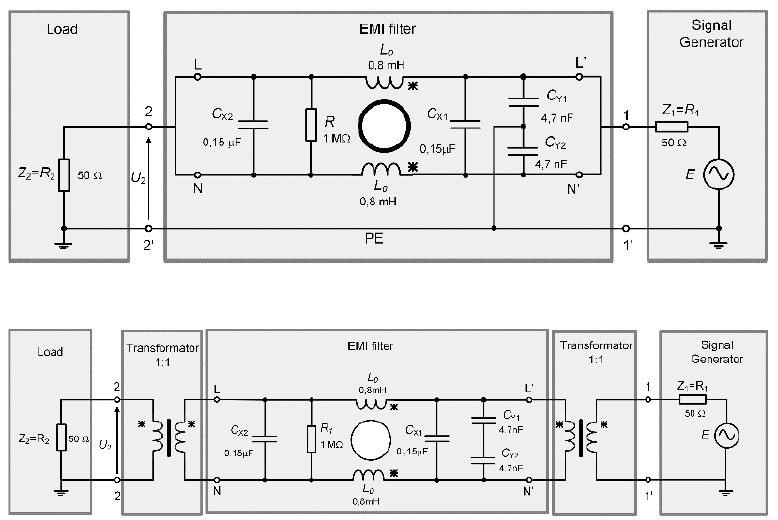
\includegraphics[width=10cm]{titelBild.png}
\end{figure}
\vfill

{
\renewcommand\arraystretch{2}
\begin{center}
\begin{tabular}{ >{\bf} l p{10cm} l }
Hochschule&Hochschule für Technik - FHNW\\
Studiengang&Elektro- und Informationstechnik\\
Auftraggeber&Dr. Luca Dalessandro\\
Betreuer&Prof. Dr. Sebastian Gaulocher \newline Prof. Peter Niklaus \newline Prof. Dr. Richard Gut \newline  Dr. Anita Gertiser \newline Pascal Buchschacher \\
Autoren&\textbf{Gruppe 1} \newline Niklaus Schwegler \newline Lukas von Däniken \newline Pascal Puschmann \newline Alfare Claudio \newline Simon Rohrer \\
Version&1.0 %Normally not used!
\end{tabular}
\end{center}
}

\clearpage

%\selectlanguage{ngerman}				%ngerman or english
\thispagestyle{empty}
			
%%---TABLE OF CONTENTS-------------------------------------------------------------------
\pagenumbering{Roman}		
%\selectlanguage{ngerman}				%ngerman or english
\tableofcontents
\clearpage

%%---TEXT--------------------------------------------------------------------------------
\pagenumbering{arabic}
\section{Übersicht} \label{sec:uebersicht}
\subsection{Ausgangslage}

In der modernen Gesellschaft hängen von Jahr zu Jahr mehr elektrische Verbraucher am Stromnetz. Der stetig steigende Leistungsbedarf dieser Verbraucher führt dazu, dass ihre Versorgung angepasst werden muss. Aus dem konventionellen Trafo-Netzteil entstand das sogenannte Schaltnetzteil. Dieses hat grosse Vorteile gegenüber dem Trafo-Netzteil, sowohl wirtschaftlich gesehen, als auch leistungsbezogen. \\Allerdings haben sie auch einen Nachteil. Sie lassen hochfrequente Störungen (EMI), entstehen, welche ins Netz zurückfliessen. Diese Störungen, welche man als Gleichtakt- und Gegentaktrauschen bezeichnet, können wiederum in anderen Verbrauchern  Störungen verursachen. \\Aufgrund dieses Problems wurden verschiedene Normen an Geräte gestellt um diese Emissionen zu minimieren. Daher werden in moderne Schaltnetzteile EMI-Filter verbaut.  Diese, auch Netzfilter genannt, bestehen aus einem Netzwerk von  aus Widerständen, Kondensatoren und Spulen. Da im Schaltnetzteil die Netzfrequenz in eine hochfrequente Spannung gewandlet wird, reagieren die Bauteile als Impedanzen und sie filtern, je nach Bauform, verschiedene hochfrequente Signale aus der Rückspeisung.


Der Auftrag von Dr. Dalessandro lautet eine Applikation zu entwickeln, welche in der Entwicklung von solchen Filtern eingesetzt werden kann. Die Anforderungen an die Applikation sind, dass die Dämpfungseigenschaften des Filters simuliert und graphisch angezeigt werden können. Dabei sollen die Gleichtakt- und die Gegentaktstörungen differenziert betrachtet weden können. Ebenfalls soll die Applikation in der Lage sein, die parasitären Einflüsse der einzelnen Parameter (Bauteile) um ± 30 \% zu variieren.   


Dieses Pflichtenheft beschreibt die technischen Aspekte des Auftrags und liefert bereits Ideen betreffend der Umsetzung. 
 

\newpage
\subsection{Projektziele} \label{subsec:projektziele}


In der Folgenden Tabelle werden alle Ziele aufgeleistet. In Kapitel 2 werden sie ausformuliert und ihre Implementation wird erläutert. 
\newcommand{\HY}{\hyphenpenalty = 25\exhyphenpenalty = 25}
\begin{table}[H]
\small
\begin{tabular}{>{\HY\RaggedRight}p{7cm} >{\HY\RaggedRight}p{1.5cm} >{\HY\RaggedRight}p{1.5cm} >{\HY\RaggedRight}p{3cm}}
\hline
\textbf{Ziel}					&\textbf{Muss}	&\textbf{Soll}	&\textbf{Zielbezeichnung}			\\						
\hline
\rowcolor{hellgrau}
\multicolumn{4}{l}{\textbf{Fachliche Anforderung}}\\
Unabhängigkeit von Betriebssystemen		&\ x &\  &\ F1\\
Modular aufgebaut/erweiterbar		&\ x &\  &\ F2\\
Berechnungen und GUI getrennt		&\ x &\  &\ F3\\
 Berechnungszeit < 10 Sek.		&\ x &\  &\ F4\\
Unabhängige Komponenten		&\   &\ x &\ F5\\
Verstellbare Parameter		&\ x &\   &\ F6\\
Verschiedene Berechnungsmodi		&\ x &\   &\ F7\\	
Monte-Carlo Simulation &\   &\ x &\ F8\\

\rowcolor{hellgrau}
\multicolumn{4}{l}{\textbf{Graphische Anforderungen}}\\			
Visualisierung der Schaltung		&\  &\ x &\ G1\\	
Einfache und schnelle Eingabemöglichkeit &\ x &\  &\ G2\\
Darstellung im Frequenzbereich bis 30MHz		&\ x &\  &\ G3\\
Mehrere Plots gleichzeitig		&\ x &\  &\ G4\\
Auslagern des Plots		&\   &\ x &\ G5\\


\rowcolor{hellgrau}
\multicolumn{4}{l}{\textbf{Anforderungen an die Bedienung}}\\			
Schutz vor Fehleingaben		&\ x &\   &\ B1\\
Export von Plots		&\  &\ x &\ B2\\
Speicherverwaltung		&\   &\ x &\ B3\\
Import von Daten		&\   &\ x &\ B4\\	
				
\hline
\end{tabular}
\end{table}

\newpage
\subsection{Lieferobjekte} \label{subsec:lieferobjekt}

Nachfolgend werden alle Lieferobjekte aufgelistet:

\newcommand{\HE}{\hyphenpenalty = 25\exhyphenpenalty = 25}
\begin{table}[H]\label{tab:lieferobjekte}
\small
\begin{tabular}{>{\HE\RaggedRight}p{5.5cm} >{\HE\RaggedRight}p{4cm} }
\hline
\rowcolor{hellgrau}
\textbf{Beschreibung}					&\textbf{Datum}			\\						
\hline
%\rowcolor{hellgrau}
%\multicolumn{2}{l}{\textbf{Objekt} } {\textbf{Datum}}\\
1. Organisatorisches Pflichtenheft		&\ 24.03.19 und 04.04.19\\
2. Technisches Pflichtenheft		&\ 24.03.19 und 04.04.19\\
3. Beta-Version des GUI	&\ 18.04.19\\
4. Beta-Version der Software &\ 28.04.19\\
5. Fachbericht	&\ 13.06.19\\
\hline
\end{tabular}
\end{table}

\section{Lösungskonzept} \label{sec:loesungskonzept}
\subsection{Problemstellung} \label{subsec:problemstellung}
Um eine erste Übersicht der möglichen Probleme des Lösungskonzepts zu erhalten, wurden folgende Punkte im Brainstormingverfahren zusammengetragen:
\begin{figure}[H]
	\centering
	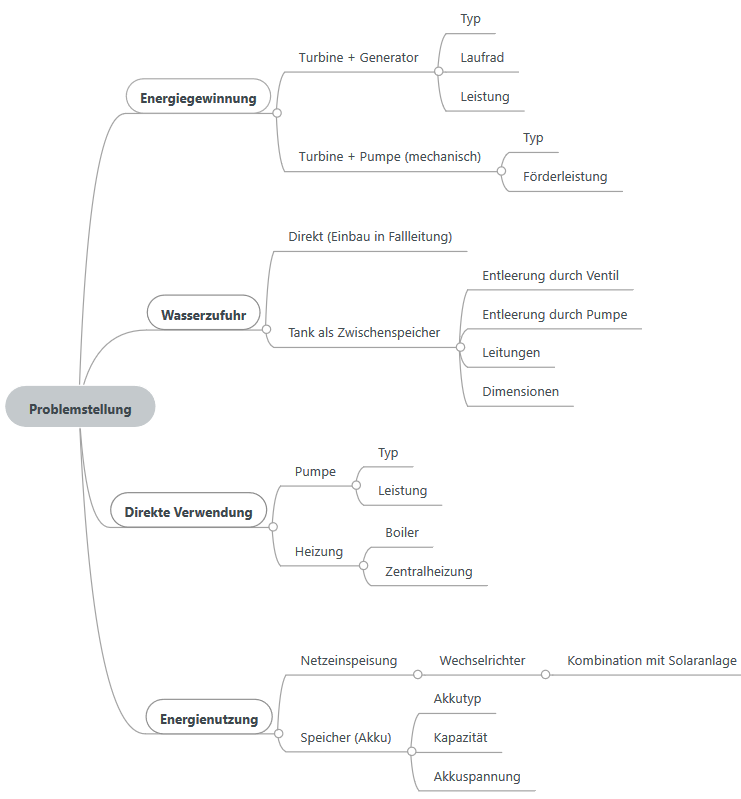
\includegraphics[width=1\linewidth]{Problemstellung_2.png}
	\caption{Baumdiagramm des Lösungskonzepts}
	\label{fig:Figure}
\end{figure}
\newpage

\subsection{Grobkonzept 1} \label{subsec:grobkonzept1}
\definecolor{dpink}{HTML}{FF13F8}
\definecolor{hpink}{HTML}{FF98FC}
\definecolor{hgruen}{HTML}{9EFFA9}
\definecolor{hblau}{HTML}{51D1FF}
\definecolor{dblau}{HTML}{008BBD}
\definecolor{hgelb}{HTML}{FFFC9E}
\definecolor{dgelb}{HTML}{FFCC67}
\definecolor{dgruen}{HTML}{00AC14}

\newcommand{\titleCell}[2]{\multicolumn{3}{c}{\cellcolor{#1}#2}}
\newcommand{\cC}[1]{\cellcolor{#1}}

%\newcommand{\HY}{\hyphenpenalty = 25\exhyphenpenalty = 25}
\begin{table}[H]
\small
\begin{tabular}{>{\HY\RaggedRight}p{3cm} >{\HY\RaggedRight}p{3.6cm} >{\HY\RaggedRight}p{6.9cm} r}
\hline
\textbf{Bestandteil}&\textbf{Typ}&\textbf{Funktion}&\textbf{Anz.}\\
\hline

\rowcolor{hellgrau}
\multicolumn{4}{l}{\textbf{Stromerzeugung}}\T\\
Wasserrad& &Umwandlung in Rotationsenergie&43\\
Generator&AC&Umwandlung in elektrische Energie&43\\
Gleichrichter&AC/DC Wandler&Wechselstrom zu Gleichstrom&43\\
DC/DC Konverter&&Regelt die Spannung für den DC Bus&43\\
Wechselrichter&&Umwandlung DC in AC (230V) &1\B\\

\rowcolor{hellgrau}
\multicolumn{4}{l}{\textbf{Kontrollsystem}}\T\\
PC&&Anlagesteuerung&1\\
SPS&Beckhof&Analoge und Digitale Ein- und Ausgänge&1\B\\

\rowcolor{hellgrau}
\multicolumn{4}{l}{\textbf{Abwassertechnik}}\T\\
Bypass&Absperrklappe&Umleitung für Wartungsarbeiten und Störungen an den Wasserräder&43\B\\


\hline
\end{tabular}
\caption{Bestandteilliste Grobkonzept 1}\label{tab:BLGrobkonzept1}
\end{table}

Im Grobkonzept 1 sollen 43 Wasserräder direkt in die Fallleitung eingebaut werden. Mit jeweils einem Generator pro Wasserrad wird Strom erzeugt. Damit der Strom der einzelnen Wasserräder zusammengeführt werden kann, muss der Wechselstrom zuerst in Gleichstrom umgewandelt werden. Dieser wird auf einen DC-DC Konverter gelegt. Anschliessend wird der Gleichstrom mit einem Wechselrichter auf die Netz-Spannung umgewandelt. Ein Kontrollsystem steuert die Anlage, überwacht die Energiegewinnung und schreitet bei Störungen ein. In unserem Hochhausmodell (Park Avenue 432) wird immer nach zwei Etagen ein Wasserrad eingebaut, um die maximale Leistung herausholen zu können. 
\newpage
\begin{wrapfigure}{r}{0.5\textwidth}
  \begin{center}
    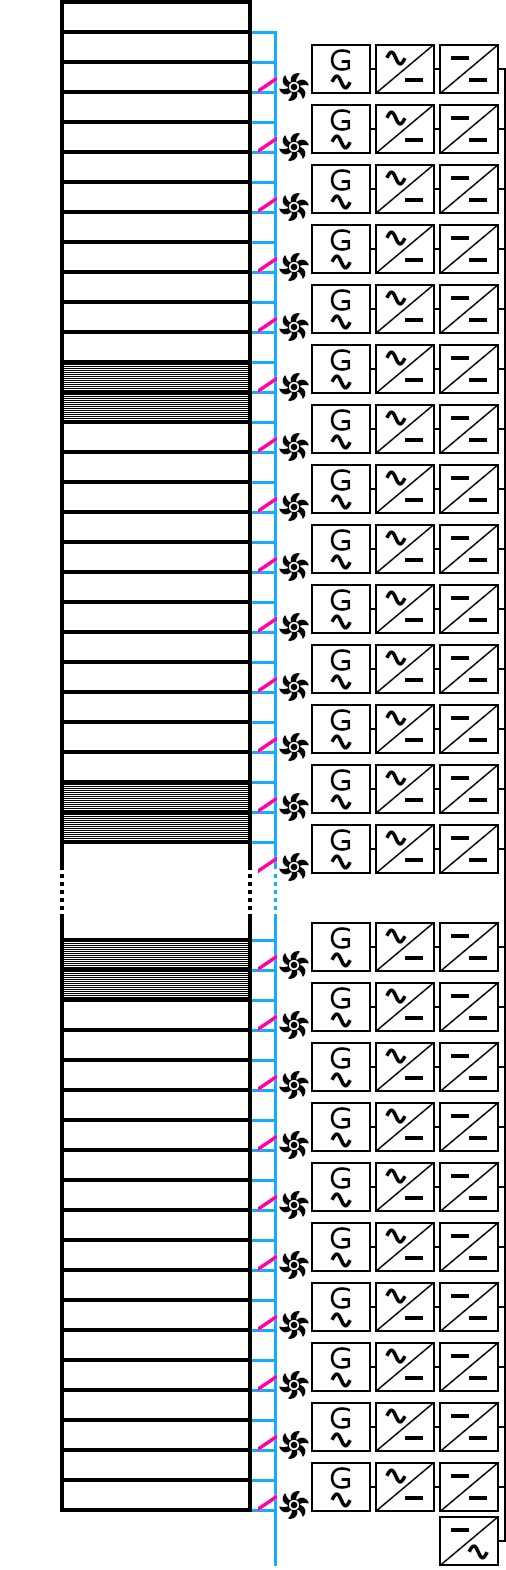
\includegraphics[width=0.48\textwidth]{grobkonzept1}
  \end{center}
  \caption{Schema Grobkonzept 1}
\end{wrapfigure}
\bigskip

\textbf{Vorteile:}								\newline
+	platzsparend									\newline
+	keine zusätzlichen Leitungen
	
\textbf{Nachteile:}								\newline
-	Luftwiderstand								\newline
- 	defektanfällig								\newline
-	AC-DC-AC Umwandlung							\newline
\WFclear
\newpage



\subsection{Grobkonzept 2} \label{subsec:grobkonzept2}
\begin{table}[H]
\small
\begin{tabular}{>{\HY\RaggedRight}p{3cm} >{\HY\RaggedRight}p{3.6cm} >{\HY\RaggedRight}p{6.9cm} r}
\hline
\textbf{Bestandteil}&\textbf{Typ}&\textbf{Funktion}&\textbf{Anz.}\\
\hline

\rowcolor{hellgrau}
\multicolumn{4}{l}{\textbf{Stromerzeugung}}\T\\
Turbine&Pelton&Umwandlung in Rotationsenergie&1\\
Generator&AC&Umwandlung in elektrische Energie&1\\
Wechselrichter&&Einspeisung ins Stromnetz&1\B\\

\rowcolor{hellgrau}
\multicolumn{4}{l}{\textbf{Kontrollsystem}}\T\\
PC&&Anlagesteuerung&1\\
SPS&Beckhof&Analoge und Digitale Aus- und Eingänge&1\B\\

\rowcolor{hellgrau}
\multicolumn{4}{l}{\textbf{Abwassertechnik}}\T\\
Tanks&&Zwischenspeicher für Abwasser&5\\
Ablassventil&&Entlässt das Abwasser aus dem Tank&5\\
Entlüftung&&Ermöglicht Luftaustausch, entlässt Gase&5\\
Notüberlauf&&Verhindert, dass Tank zu voll wird&5\\
Füllstandsensor&Vibronik Grenzschalter &Misst den Füllstand des Tanks&5\\
Druckleitungen&&Können Druck standhalten&5\\
Bypass für Turbine&&Ermöglicht Wartung der Turbine&1\\
Bypass für Tanks&&Ermöglicht Wartung \& Reingung der Tanks&5\\
Einwegventile&&Verhindern Rückfluss&4\B\\
\hline
\end{tabular}
\caption{Bestandteilliste Grobkonzept 2}\label{tab:BLGrobkonzept2}
\end{table}
Im Grobkonzept 2 soll die Energieausbeutung gesteigert werden, indem das Abwasser zuerst in Tanks gespeichert wird, die all 14 Stockwerke eingebaut sind. In unserem Hochmausmodell (Park Avenue 432) gibt es nach 12 Stockwerken jeweils zwei Zwischenstockwerke, wo der Einbau möglich wäre. Wenn der Füllstandsensor im Tank erkennt, dass er voll ist, wird das Ventil geöffnet und das Abwasser fliesst durch die Druckleitung in den Keller, wo es eine Pelton-Turbine mit Generator antreibt. Die gewonnene elektrische Energie wird über einen Wechselrichter dem Stromnetz zugeführt. \\ 
Das Abwasser füllt das Rohr komplett, so dass es keinen Luftwiderstand gibt, der es abbremst. So kann der Wirkungsgrad des Systems verbessert werden. Nur für eine Kurze Zeit, bis das Rohr komplett mit Wasser gefüllt ist, tritt Luftwiderstand auf.\\
Da es im Modellhochhaus in den letzten 17 Stockwerken kein Zwischenstockwerk mehr gibt, bleibt das Abwasser dieser Stockwerke ungenutzt.\\
Die baulichen Massnahmen, die nötig sind, um dieses System zu installieren sind beträchtlich. Es müssen Tanks eingebaut und Druckleitungen zur Turbine verlegt werden, welche im Keller installiert werden muss. Die bestehenden Abwasserleitungen müssen neu so verlegt werden, dass sie in die Tanks führen. Somit ist es eher für Neubauten geeignet als zur Nachrüstung.
\newpage

\begin{wrapfigure}{r}{0.5\textwidth}
  \begin{center}
    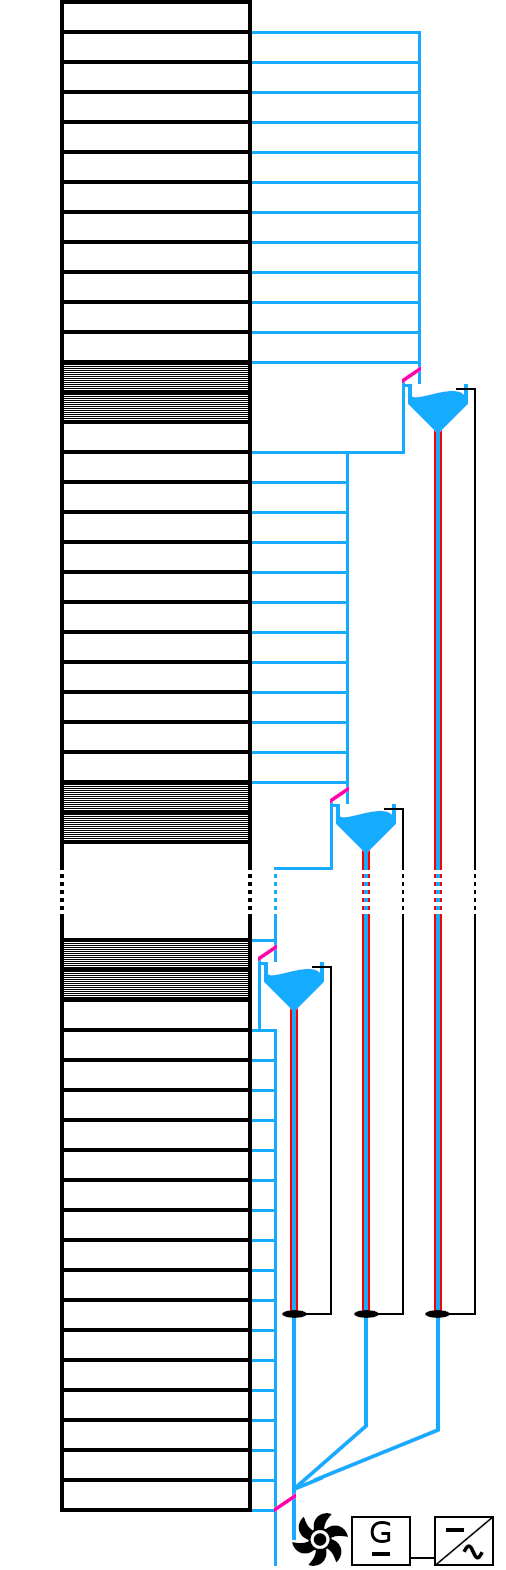
\includegraphics[width=0.48\textwidth]{grobkonzept2}
  \end{center}
  \caption{Schema Grobkonzept 2}
\end{wrapfigure}




Um zu verhindern, dass es in den Tanks zu Ablagerungen kommt, ist der Boden der Tanks trichterförmig. Ablagerungen werden dadurch beim Öffnen des Ventils weggespült. Sollte es trotzdem nötig sein, die Tanks zu reinigen, gibt es einen Bypass, mit dem das Abwasser am Tank vorbeigeführt werden kann.
Er kann dann entleert und gereinigt oder repariert werden. Auch die Turbine hat einen Bypass, der Wartungsarbeiten ermöglicht.

Jeder Tank ist mit einem Überlauf ausgestattet, der verhindert, dass ein Tank zu voll wird wenn z.B. der Ablauf verstopft ist. Das überschüssige Abwasser wird dann in einem Rohr in die Fallleitung wenige Stockwerke tiefer geleitet. Von dort gelangt es in den nächsten Abwassertank. Der Füllstandsensor im Tank erkennt, wenn der Pegel zu hoch wird und sendet eine Warnung.
Falls aus irgendeinem Grund mehr als eines der Ventile gleichzeitig geöffnet würde, könnte es zu einem Rückstau kommen, bei dem Abwasser durch die Druckleitungen vom höher gelegenen Tank in einen tieferen fliesst. Um dies zu verhindern, werden in den Druckleitungen Einwegventile eingebaut. Der höchstgelegene Tank benötigt kein solches Ventil. 

Ein Kontrollsystem steuert die Anlage und überwacht die Energiegewinnung und schreitet bei Störungen ein. Die Gewonnene Energie kann ins Netz zurück gespeist werden.

\bigskip

\textbf{Vorteile:} 									\newline
+	Luftwiderstand nur während Füllung				\newline
+	Nur eine Turbine									\newline
+	Keine AC-DC-AC Umwandlung						\newline
+	geregelte Wasserflussmenge						\newline

\textbf{Nachteile:}									\newline
-	braucht sehr viel Platz 							\newline
-	bauliche Massnahmen								\newline
-	Luftwiderstand während Füllung					\newline
- 	lange Druckleitungen								\newline
-	Abwasser der untersten 17 Stockwerke ungenutzt	\newline
\WFclear

\subsection{Grobkonzept 3} \label{subsec:grobkonzept3}
\begin{table}[H]
\small
\begin{tabular}{>{\HY\RaggedRight}p{3cm} >{\HY\RaggedRight}p{3.6cm} >{\HY\RaggedRight}p{6.9cm} r}
\hline
\textbf{Bestandteil}&\textbf{Typ}&\textbf{Funktion}&\textbf{Anz.}\\
\hline

\rowcolor{hellgrau}
\multicolumn{4}{l}{\textbf{Stromerzeugung}}\T\\
Turbine&Pelton&Umwandlung in Rotationsenergie&5\\
Generator&AC&Umwandlung in elektrische Energie&5\\
Gleichrichter&AC/DC Wandler&Wechselstrom zu Gleichstrom&5\\
DC/DC Konverter&&Regelt die Spannung für den DC Bus&5\\
Wechselrichter&&Umwandlung DC in AC (230V)&1\B\\

\rowcolor{hellgrau}
\multicolumn{4}{l}{\textbf{Kontrollsystem}}\T\\
PC&&Anlagesteuerung&1\\
SPS&Beckhof&Analoge und Digitale Ein- und Ausgänge&1\B\\

\rowcolor{hellgrau}
\multicolumn{4}{l}{\textbf{Abwassertechnik}}\T\\
Tanks&&Zwischenspeicher für Abwasser&5\\
Ablassventil&&Entlässt das Abwasser aus dem Tank&5\\
Entlüftung&&ermöglicht Luftaustausch, entlässt Gase&5\\
Notüberlauf&&Verhindert, dass Tank zu voll wird&5\\
Füllstandsensor&Vibronik Grenzschalter&Misst den Füllstand des Tanks&5\\
Druckleitungen&&Können Druck standhalten&5\\
Bypass für Turbine&&ermöglicht Wartung der Turbine&5\\
Bypass für Tanks&&ermöglicht Wartung \& Reingung der Tanks&5\B\\ 
\hline
\end{tabular}
\caption{Bestandteilliste Grobkonzept 3}\label{tab:BLGrobkonzept3}
\end{table}
Dieses Grobkonzept ist fast identisch zu Grobkonzept 2. Es gibt wieder mehrere Tanks in einem Abstand von 14 Stockwerken, in denen das Abwasser zwischengespeichert wird. Allerdings gibt es nicht nur eine, sondern gleich viele Turbinen wie Tanks. Das Abwasser fliesst von einem Tank 14 Stockwerke nach unten, durch eine Turbine und dann in den nächsten Tank. Bei Grobkonzept 2 kann es unter Umständen relativ lange dauern, bis die Rohre komplett mit Wasser gefüllt sind. Bis das der Fall ist, kommt es zu Luftwiderstand in der Leitung, der das Abwasser abbremst. Bei jedem Tank eine Turbine einzubauen hat den Vorteil, dass die Rohre kürzer sind und so nach öffnen des Ventils schneller komplett mit Wasser gefüllt werden. So wird die Zeit verkürzt, in der Luftwiderstand auftritt. Ausserdem ist der Druck in den Leitungen geringer, man kann also günstigere Rohre und Ventile verwenden. Da im Vergleich zu Grobkonzept 2 keinen Rückstau geben kann, ist es nicht nötig, Einwegventile in die Druckleitung einzubauen. 
Damit der Strom der Turbinen zusammengeführt werden kann, muss der Wechselstrom zuerst in Gleichstrom umgewandelt werden. Dieser wird auf einen DC-DC Konverter gelegt damit kein Strom zurück in den Generator fliessen kann.
\newpage
\begin{wrapfigure}{r}{0.5\textwidth}
  \begin{center}
    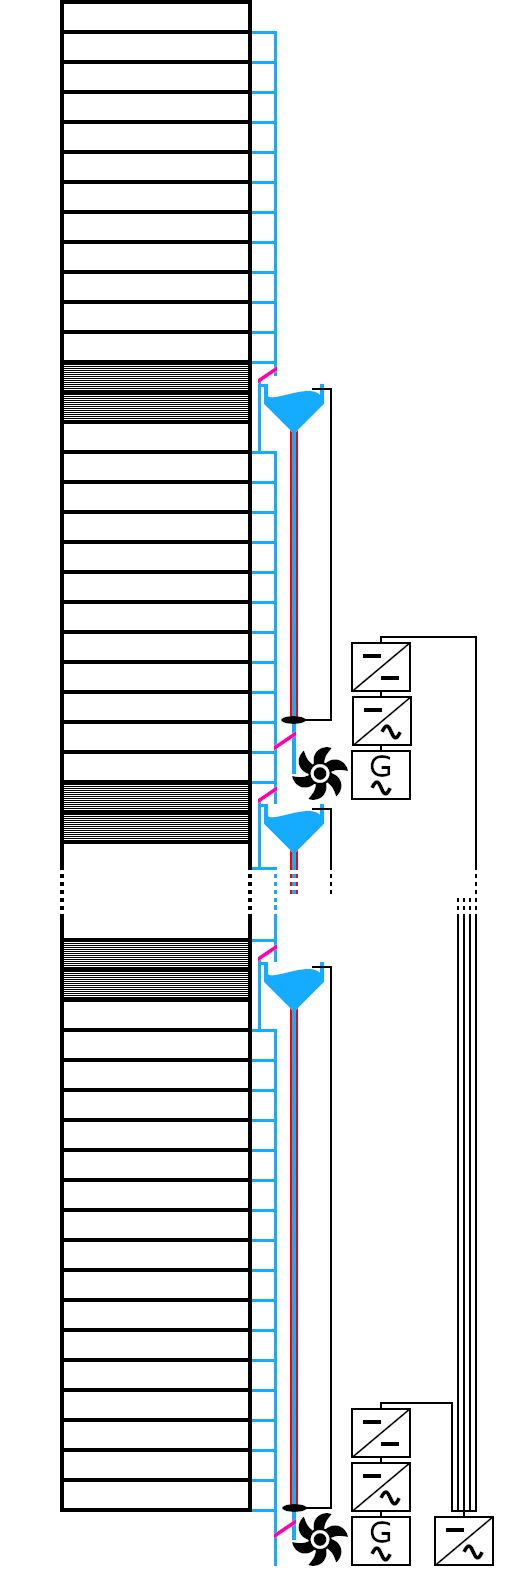
\includegraphics[width=0.48\textwidth]{grobkonzept3}
  \end{center}
  \caption{Schema Grobkonzept 3}
\end{wrapfigure}

Anschliessend wird der Gleichstrom mit einem Wechselrichter auf Netz-Spannung umgewandelt.

Ein Kontrollsystem steuert die Anlage und überwacht die Energiegewinnung und schreitet bei Störungen ein.

\textbf{Vorteile:} 									\newline
+	Luftwiderstand nur während Füllung				\newline
+	kurze Druckleitungen								\newline
+	geregelte Wasserflussmenge						\newline

\textbf{Nachteile:}									\newline
-	Braucht viel Platz								\newline
-	grössere bauliche Massnahmen						\newline
-	Mehrere Turbinen									\newline
-	AC-DC-AC Umwandlung								\newline
-	Abwasser der untersten 17 Stockwerke ungenutzt	\newline
\WFclear			
\newpage

\subsection{Grobkonzept 4} \label{subsec:grobkonzept3}
\begin{table}[H]
\small
\begin{tabular}{>{\HY\RaggedRight}p{3cm} >{\HY\RaggedRight}p{3.6cm} >{\HY\RaggedRight}p{6.9cm} r}
\hline
\textbf{Bestandteil}&\textbf{Typ}&\textbf{Funktion}&\textbf{Anz.}\\
\hline

\rowcolor{hellgrau}
\multicolumn{4}{l}{\textbf{Stromerzeugung}}\T\\
Rohrkette&&Umwandlung potenzielle Energie zu Rotation&6\\
Zahnrad&&Umdehungszahl für Generator anpassen&6\\
Generator&AC&Umwandlung in elektrische Energie&6\\
Gleichrichter&AC/DC Wandler&Wechselstrom zu Gleichstrom&6\\
DC/DC Konverter&&Regelt die Spannung für den DC Bus&6\\
Wechselrichter&&Umwandlung DC in AC (230V)&1\B\\

\rowcolor{hellgrau}
\multicolumn{4}{l}{\textbf{Kontrollsystem}}\T\\
PC&&Anlagesteuerung&1\\
SPS&Beckhof&Analoge und Digitale Ein- und Ausgänge&1\B\\

\rowcolor{hellgrau}
\multicolumn{4}{l}{\textbf{Abwassertechnik}}\T\\
Ventile&Absperrklappe&Umleitung in Fallleitung für Wartungsarbeiten am Wasserlift&74\\
Fallleitung&&Für Wartungsarbeiten&1\B\\

\hline
\end{tabular}
\caption{Bestandteilliste Grobkonzept 4}\label{tab:BLGrobkonzept4}
\end{table}
Im Grobkonzept 4 wird die potenzielle Energie des Abwassers mit einem Wasserlift ausgenutzt. Der Lift besteht aus einer Umlaufenden Kette, an der runde, tellerförmige Schaufeln befestigt sind. Die Kette bewegt sich  durch zwei parallele, vertikal verlegte Rohre, im einen nach oben und im anderen nach unten. Am oberen und unteren Ende wird die Kette mit einem Rad in das andere Rohr umgelenkt. Das Abwasser fliesst aus dem jeweiligen Stockwerk in eine der Schaufeln und treibt den Lift durch sein Gewicht an. Das Abwasser wandert im Lift nach unten und wird am tiefsten Punkt entleert.
Die Drehbewegung, welche die Rohrkette dabei erzeugt, ist eher langsam. Daher muss die Drehzahl mit einem Getriebe erhöht werden, damit die Mindestdrehzahl des Generators erreicht wird.\\
Während Wartungsarbeiten wird das Abwasser mittels Ventilen in eine Fallleitung umgeleitet. Damit der Strom der Turbinen zusammengeführt werden kann, muss der Wechselstrom zuerst in Gleichstrom umgewandelt werden. Dieser wird auf einen DC-DC Konverter gelegt, damit kein Strom zurück in den Generator fliessen kann. Anschliessend wird der Gleichstrom mit einem Wechselrichter auf Netz-Spannung umgewandelt.\\
Ein Kontrollsystem steuert die Anlage, überwacht die Energiegewinnung und schreitet bei Störungen ein. Die 5 oberen Lifte haben eine Länge von \(66.08m\), der unterste Lift \(80.24m\). Für Wartungsarbeiten existiert eine zusätzliche Leitung, die mittels Ventilen angesteuert wird.
\newpage
\begin{wrapfigure}{r}{0.5\textwidth}
  \begin{center}
    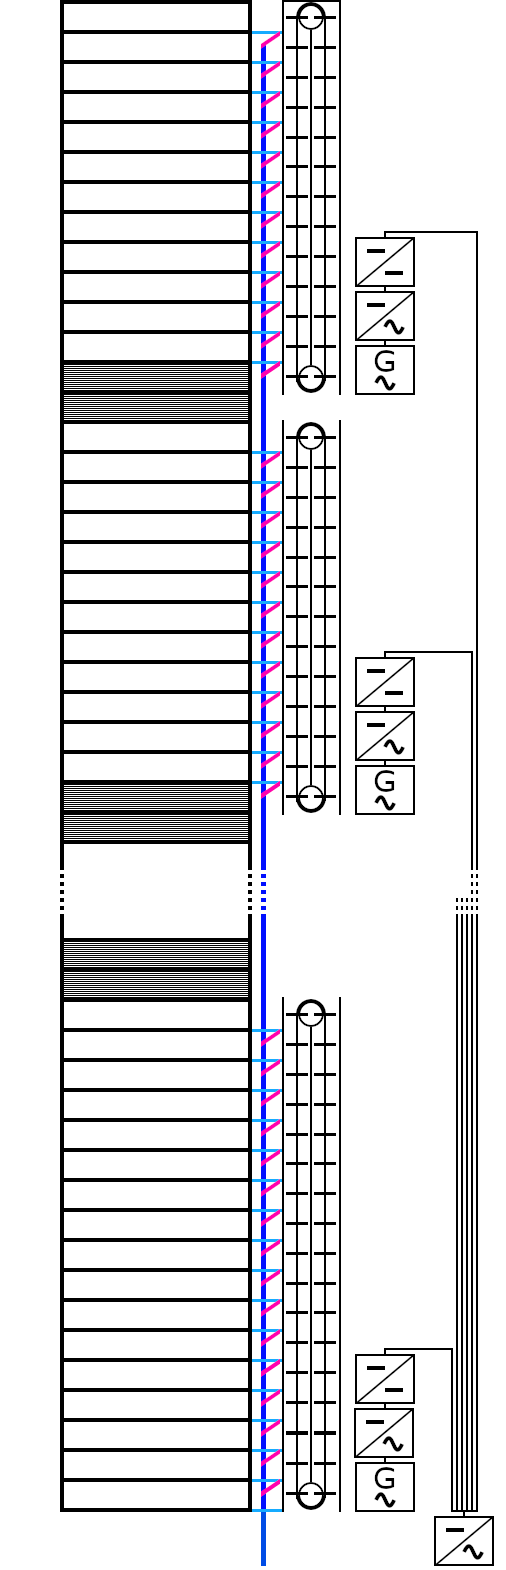
\includegraphics[width=0.48\textwidth]{grobkonzept4}
  \end{center}
  \caption{Schema Grobkonzept 4}
\end{wrapfigure}


\textbf{Vorteile:}							\newline
+ 	platzsparend								\newline
\newline
\textbf{Nachteile:}\newline
-	viele Ventile								\newline
-	Lufwiderstand							\newline
\WFclear			
\newpage








\section{Auswertung} \label{sec:auswertung}

\subsection{Modell} \label{subsec:modell}

Für die Berechnung der potentiellen Energie benützen wir das Modell Park Avenue 432, eines der höchsten reinen Wohnhochhäusern auf der Welt. Die stolze Höhe und der über das ganze Gebäude gleichbleibende quadratische Grundriss sind ideal für unsere Berechnungen. Für die Wassermengenberechnung stützen wir uns auf die Angaben des durchschnittlichen Wasserverbrauchs in Amerika pro Person und Tag: 314\si{L}. \cite{waterUsAmerica}

\begin{figure} [H]
	\centering
	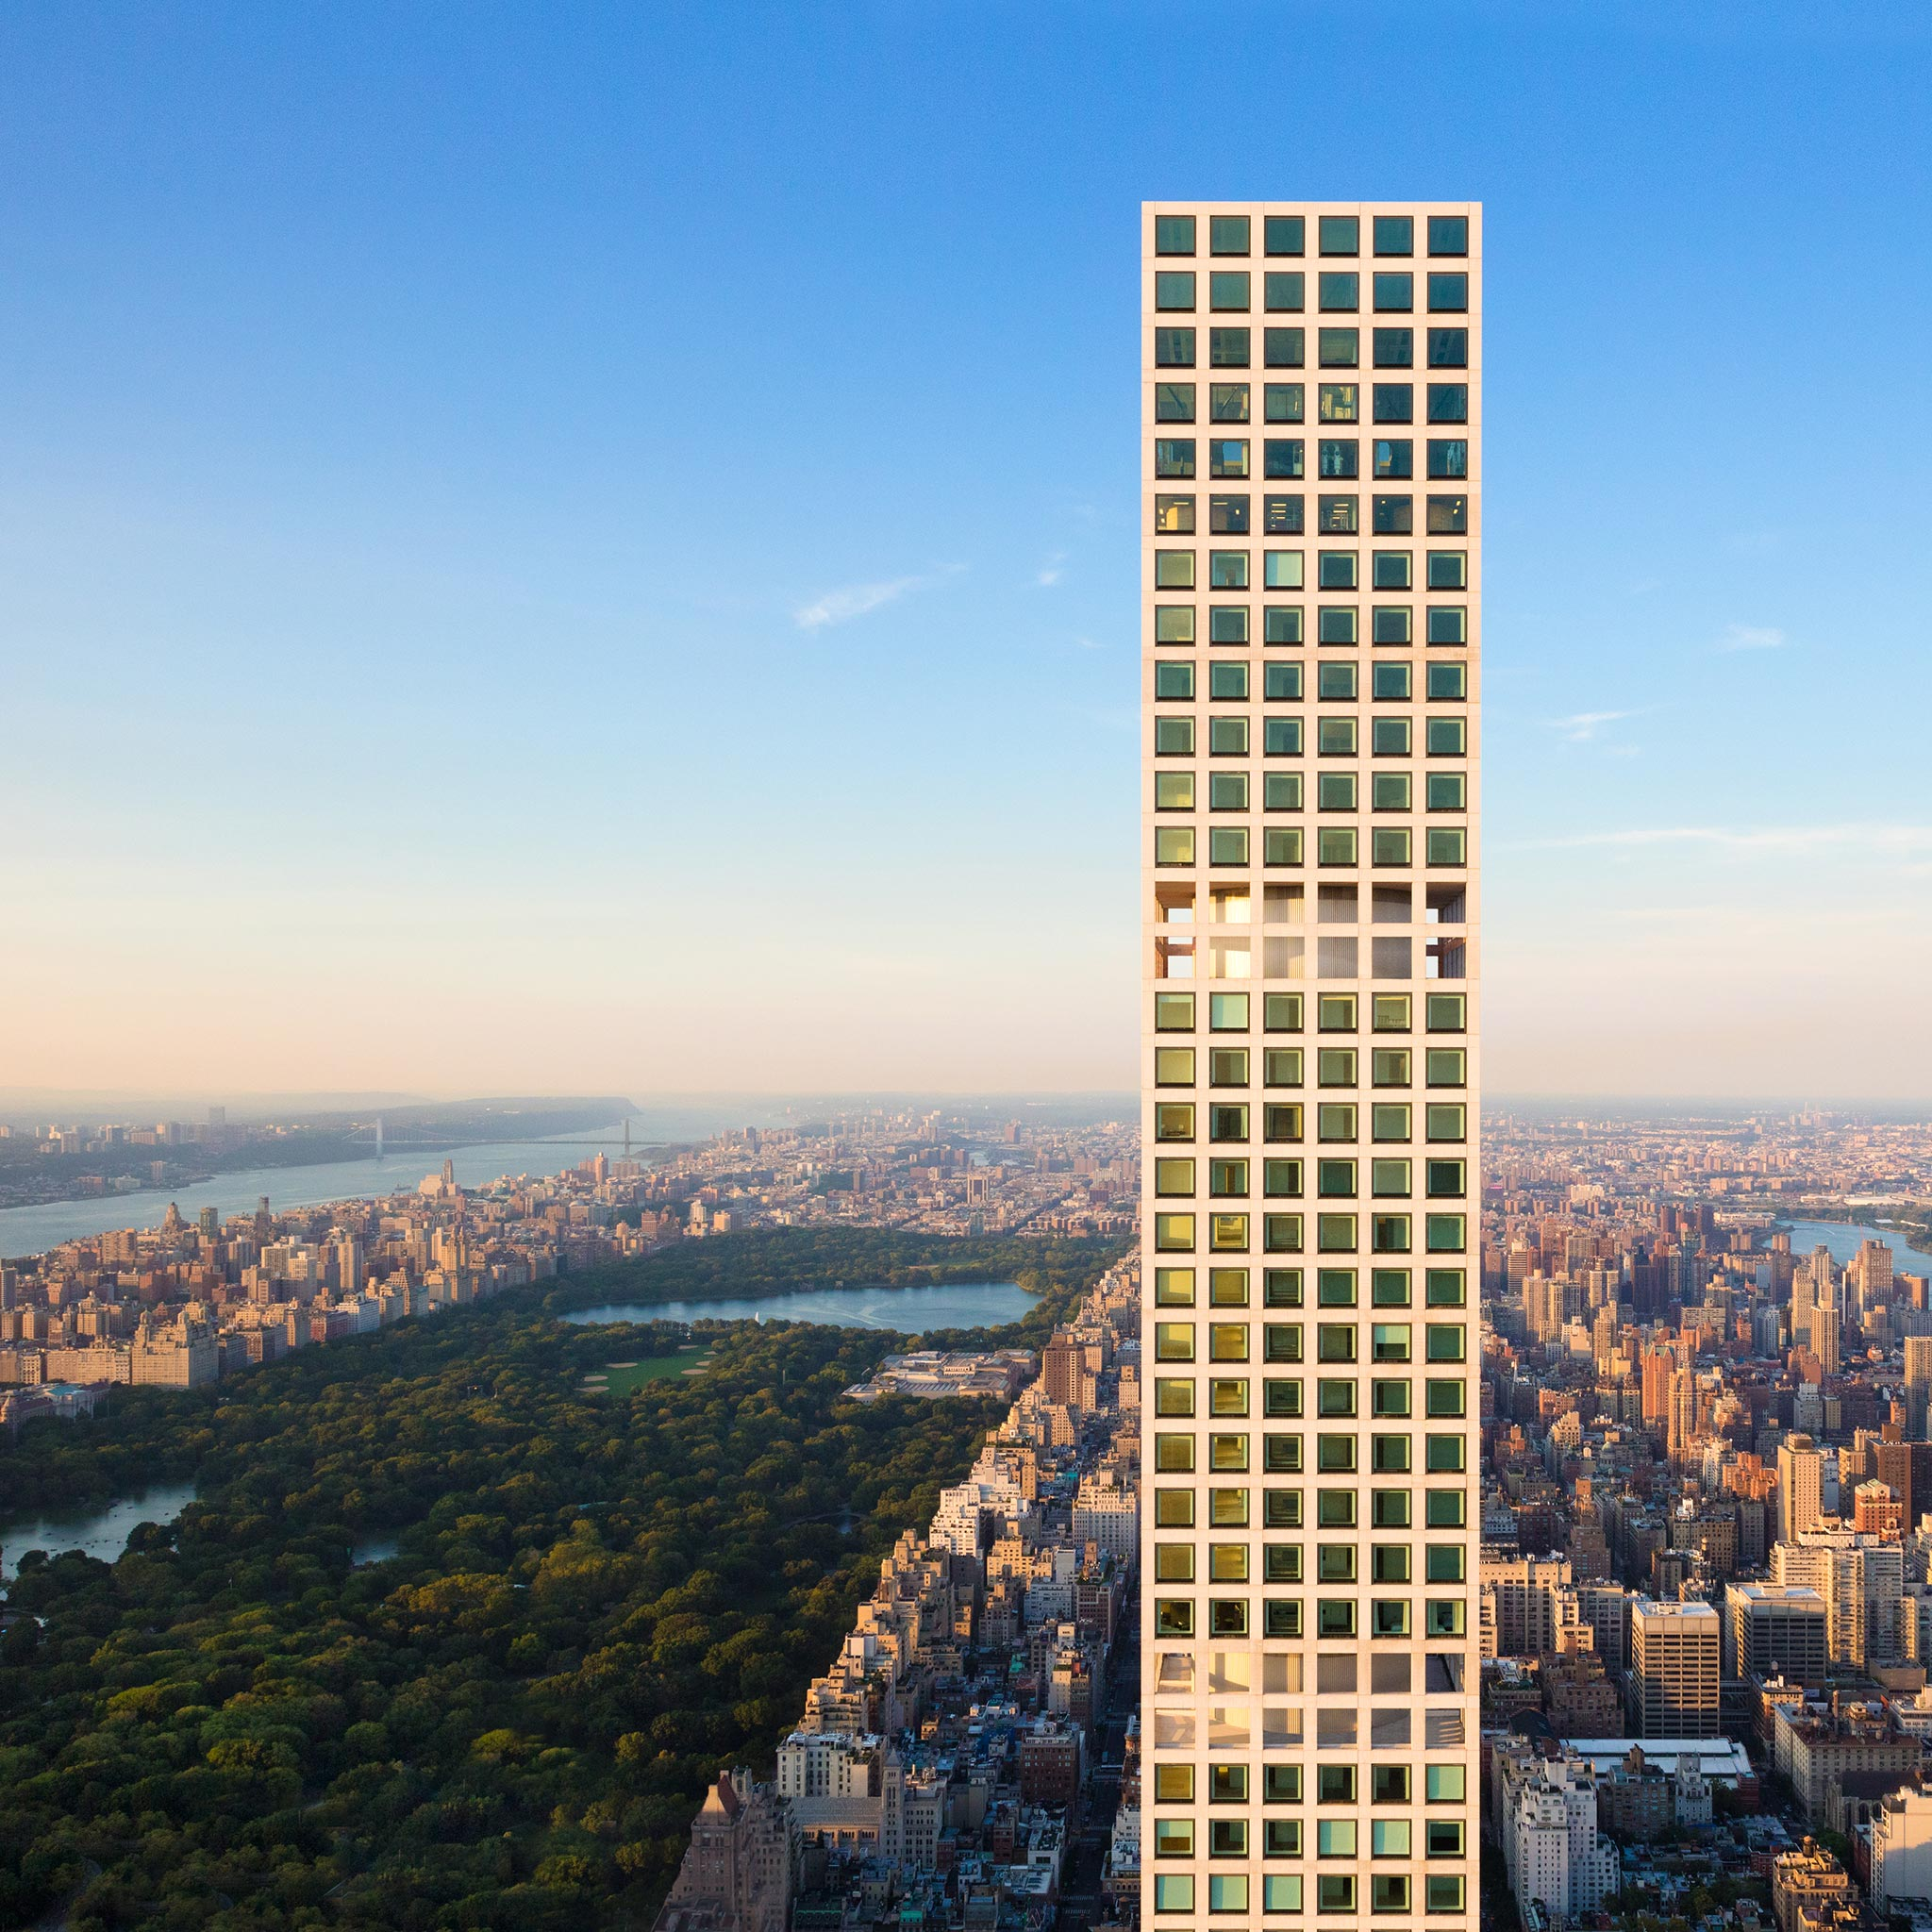
\includegraphics[width=12cm]{parkAvenue.jpg}
	\caption{Park Avenue 432 \cite{432_Park_Avenue}}
	\label{fig:Park_Avenue_432}
\end{figure}

\begin{table}[H]
\centering
\begin{tabular}{ll}
Name:				&Park Avenue 432\\
Höhe: 				&426m\\          
Etagen:				&84 Obergeschosse, 1 Erdgeschosse, 3 Untergeschosse\\
Etagenhöhe:			&4.72m\\
Höchste Etage:		&392.1m\\
Wohnungen:			&104\\
Speziell:			&alle 12 Etagen 2 Etagen leer\\    
Nutzbare Etagen: 	&74       
\end{tabular}
\end{table}

\newpage

\subsection{Energieberechnung} \label{subsec:energieberechnung}

Die Endgeschwindigkeit des Abwassers kann mit folgender Formel berechnet werden:
\begin{center}
\[
	v = \sqrt{2 \cdot g \cdot h}
\]
\end{center}

Die Einheit der Geschwindigkeit \(v\) ist \si{m/s}, das Schwerefeld \(g\) auf der Erde besitzt den Wert 9.81~\si{N/kg}, und die Höhe \(h\) hat die Einheit \si{m}.

\bigskip

Die Energie, die gewonnen werden kann, wird mit folgender Formel berrechnet:

\begin{center}
\[
	E =\frac 12\ \cdot m \cdot v^2
\]
\end{center}

Die Energie \(E\) hat die Einheit \si{J}, die Einheit der Geschwindigkeit \(v\) ist \si{m/s}, und die Masse \(m\) hat die Einheit \si{kg}

\bigskip

Um die Leistung in \si{kWh} zu erhalten wird forlgende Formel verwendet:

\begin{center}
\[
	P = \frac{E \cdot \eta}{3.6\si{MJ}}
\]
\end{center}

Die Leistung \(P\) hat die Einheit \si{W} und der Wirkungsgrad \(\eta\) besitzt keine Einheit.

\newpage

Mit diesen mathematischen Grundlagen kann nun von jedem Grobkonzept die Leistung anhand des Modellhochhauses berechnet werden. Für die Berchnungen wird angenommen, dass pro Wohnung 2.5 Personen leben und diese einen Durchschnittsverbrauch pro Tag von 785\si{L} haben. Bei 146 Wohnungen und 74 Nutzbaren Etagen leben 5 Personen pro Etage. Es wird somit 1570\si{L} pro Etage pro Tag verbraucht. Im Anhang befindet sich das vereinfachte Modell (\ref{fig:VereinfachtesModel} \nameref{fig:VereinfachtesModel}) des Hochhauses, von dem die Berechnungen ausgehen. Das gesamte Hochhaus wird zur Vereinfachung in 6 Blöcke unterteilt. Dies ist, zusammen mit einer Legende für die benutzten Symbole, in der Abbildung \ref{fig:EinteilungBloecke} \nameref{fig:EinteilungBloecke} ersichtlich.

\bigskip

\begin{figure} [H]
	\centering
	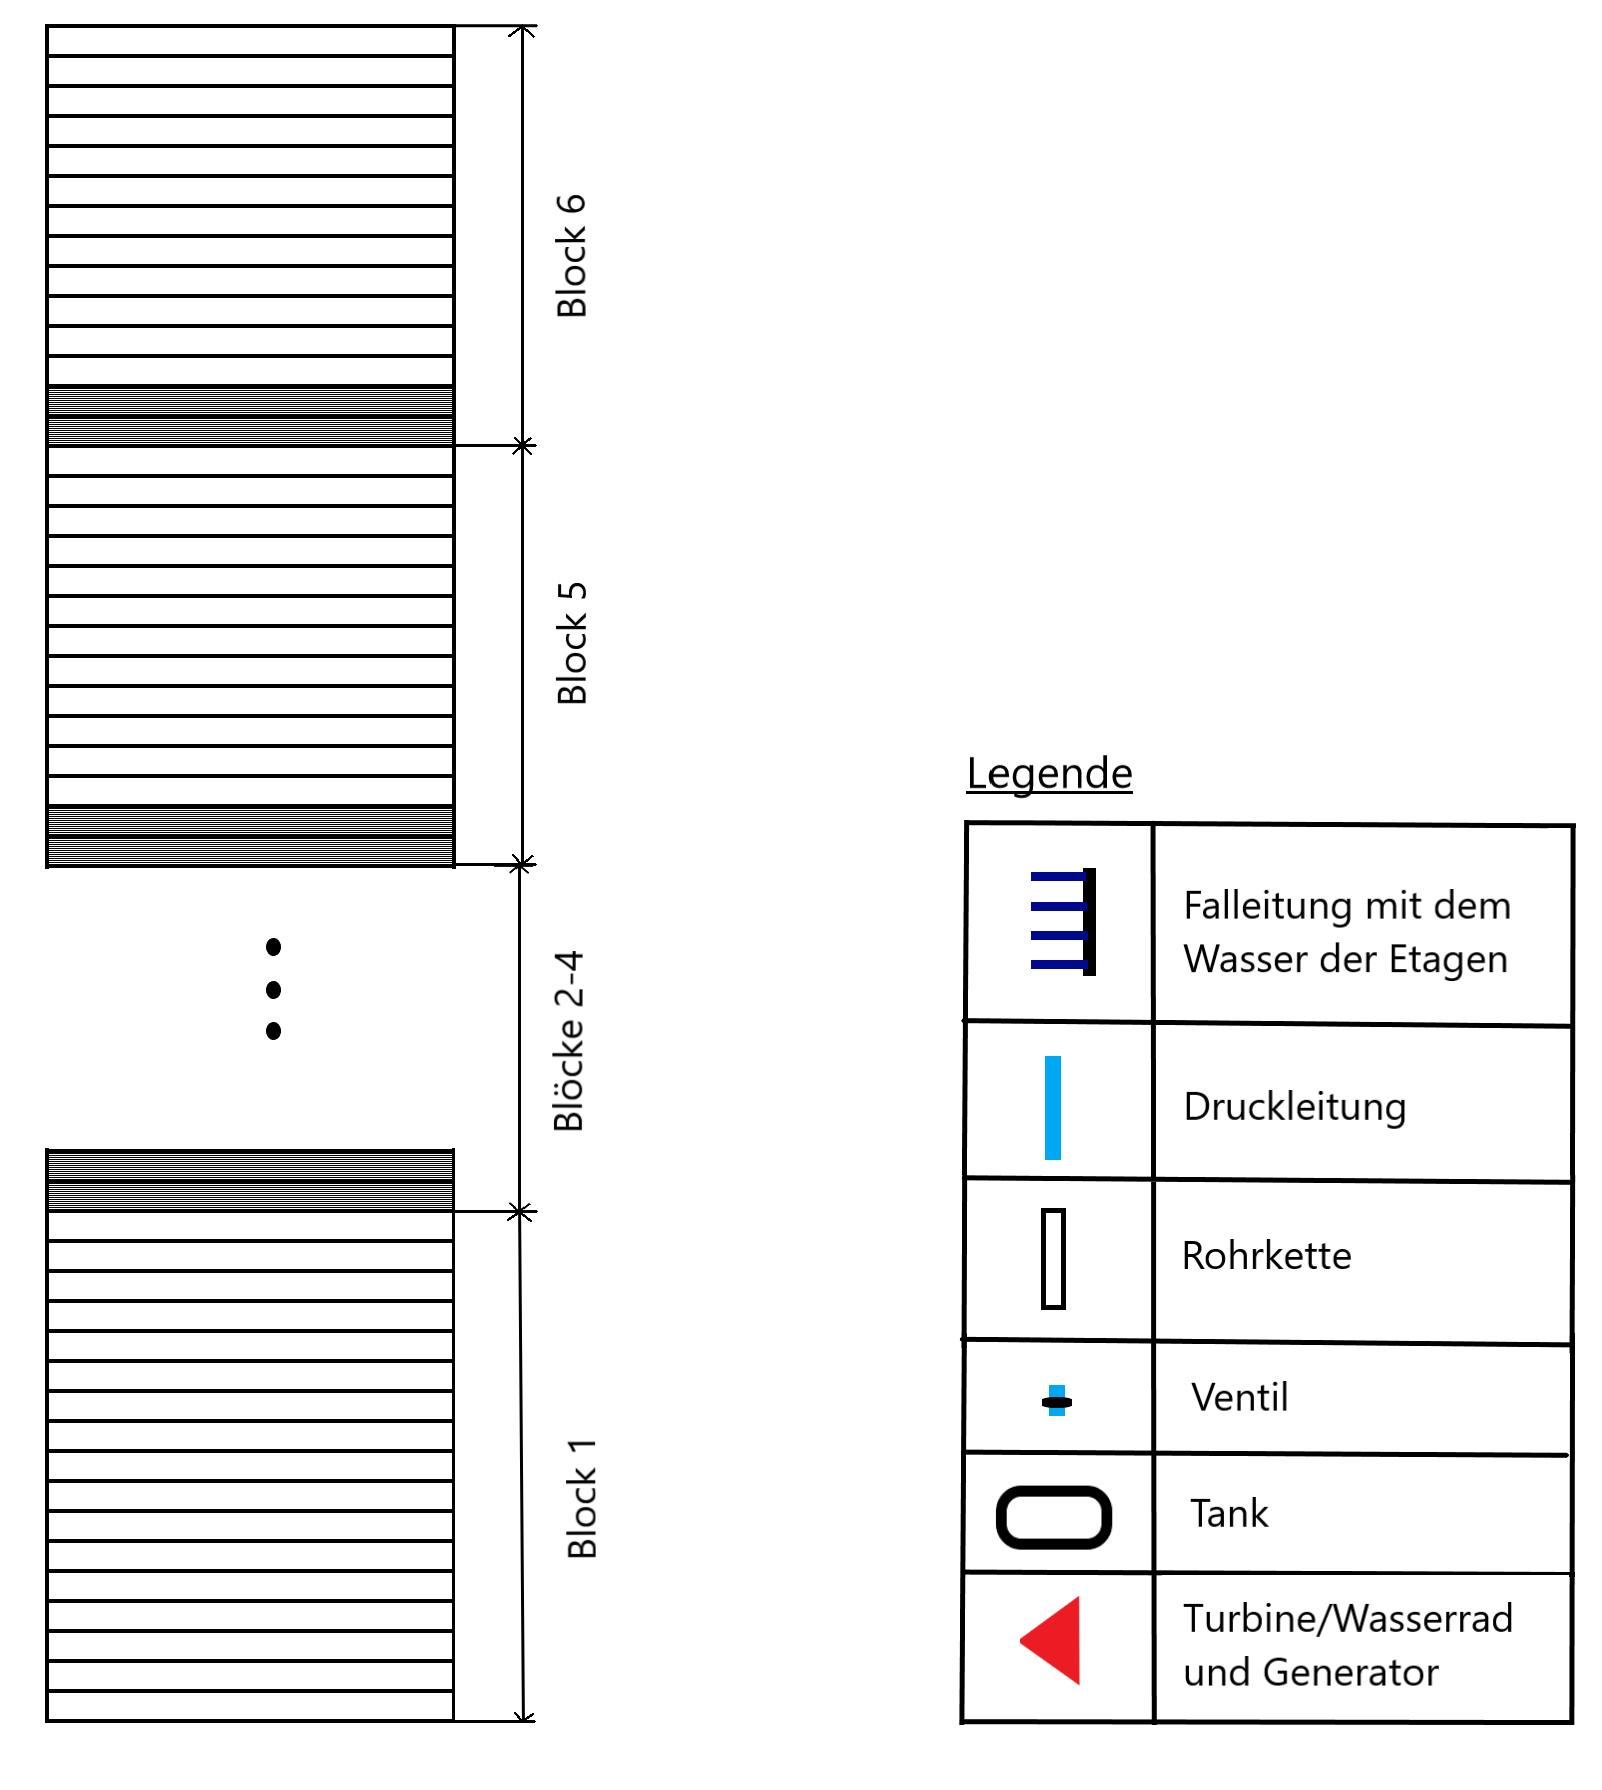
\includegraphics[width=11cm]{EinteilungBloecke.png}
	\caption{Blockeinteilung des Hochhauses}
	\label{fig:EinteilungBloecke}
\end{figure}

\newpage

\paragraph{Grobkonzept 1} 

Im Grobkonzept 1 wird die Geschwindigkeit des Abwassers ausgenutzt. Wie bereits im Recherchedokument \cite{recherchedokument} berechnet, wird das Wasser ab ca. 10m nicht mehr merklich schneller. Um möglichst viel Energie zu erzeugen wird in jeder zweiten Etage, also alle 9.44\si{m} ein kleines Wasserrad eingebaut. Ingesamt werden 43 Wasserräder eingebaut. Dies ist in der Abbildung \ref{fig:PrinzipGrobkonzept1} \nameref{fig:PrinzipGrobkonzept1} ersichtlich. Die Geschwindigkeit des Abwassers beträgt bei einer Höhe von zwei Etagen 8.5\si{m/s} und bei einer Etage 6.5\si{m/s}

\begin{figure} [H]
	\centering
	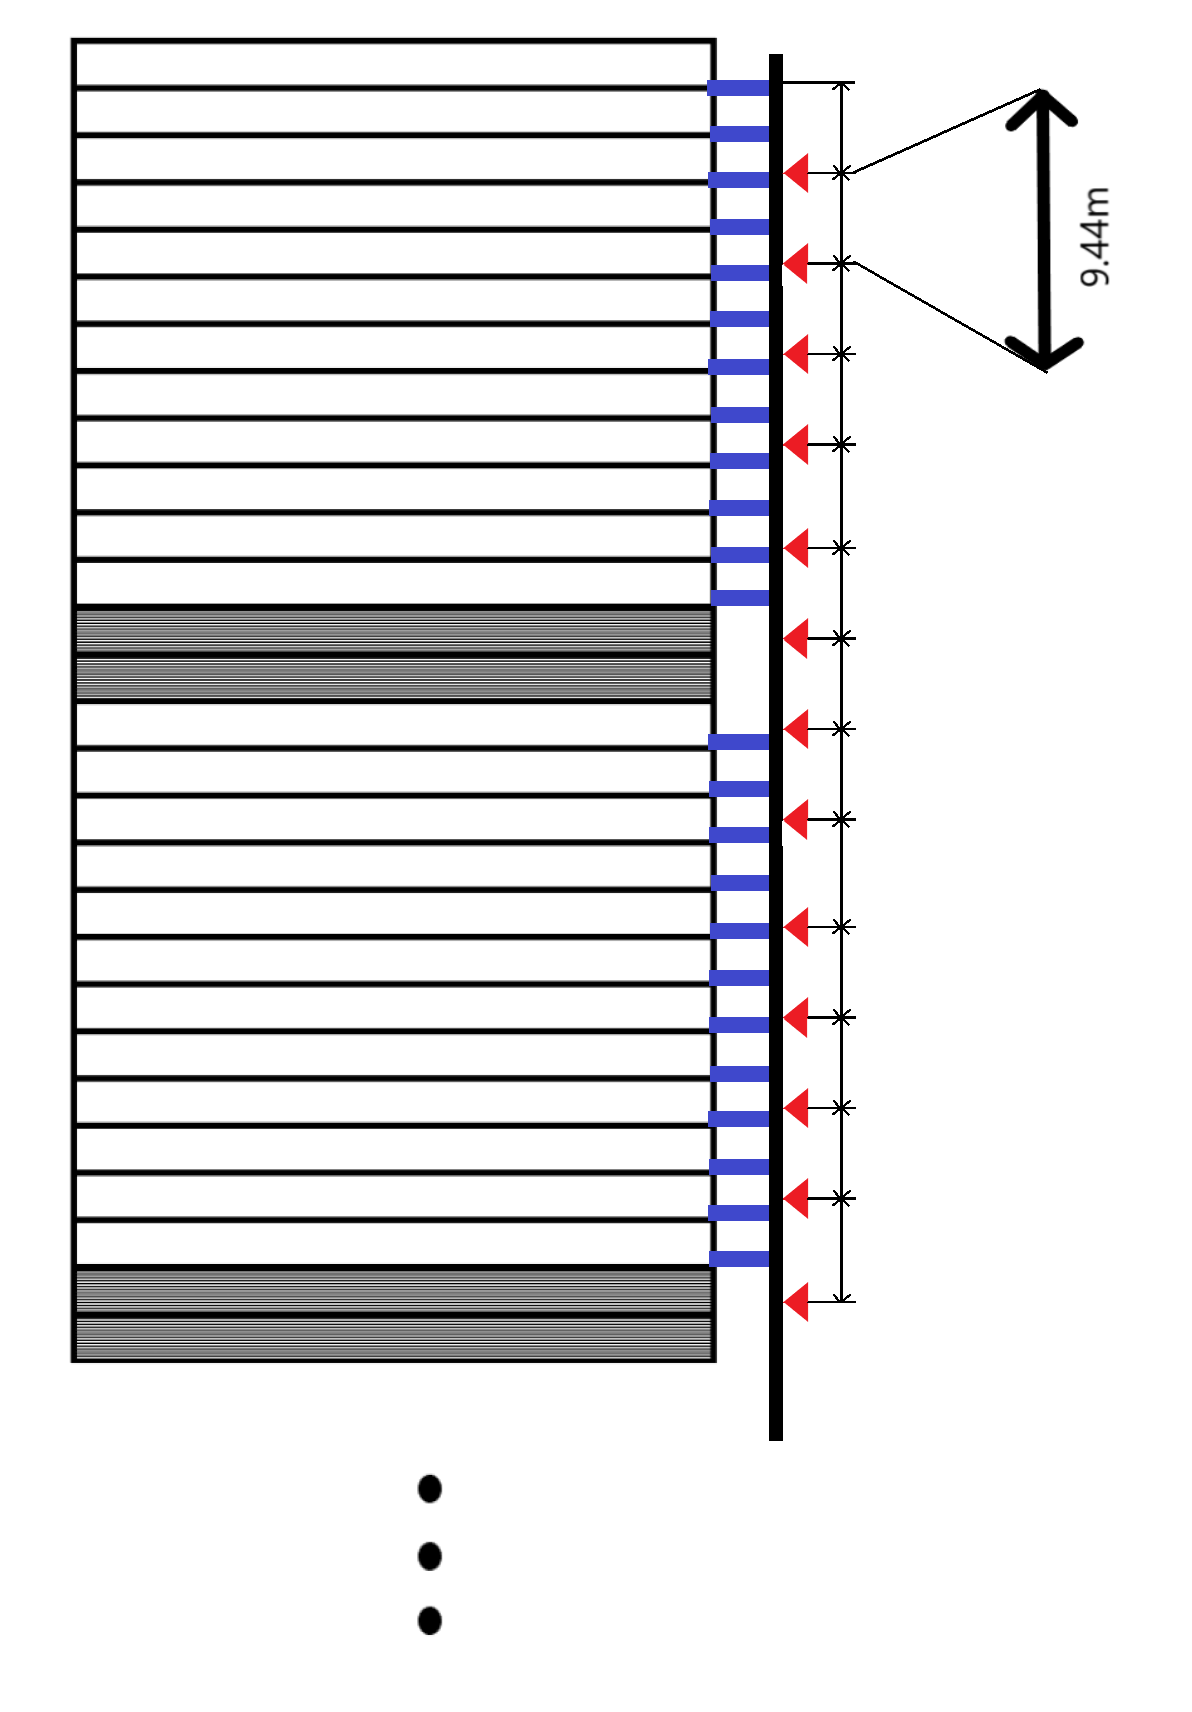
\includegraphics[width=9cm]{PrinzipGrobkonzept1.png}
	\caption{Prinzip Grobkonzep 1}
	\label{fig:PrinzipGrobkonzept1}
\end{figure}

Mit diesem Konzept wird insgesamt 21.5\si{kWh} pro Tag gewonnen, dies entspricht bei Stromkosten von 20\si{rp} einem Wert von 4.30\si{Fr}. Die Leistungsberechnungen sind im Anhang \ref{fig:BerechnungGrobkonzept1} \nameref{fig:BerechnungGrobkonzept1} zu finden.

\newpage

\paragraph{Grobkonzept 2}

Im Grobkonzept 2 wird die Geschwindigkeit des Abwassers ausgenutzt. Um den Luftwiderstand zu eliminieren, werden nun Druckleitungen eingebaut, die komplett mit Abwasser gefüllt werden. So kann eine grössere Geschwindigkeit erreicht werden. In den unbenutzen Etagen wird das Wasser gesammelt und mit einer Druckleitung bis zur Turbine ganz unten geführt. Dies ist in der Abbildung \ref{fig:PrinzipGrobkonzept2} \nameref{fig:PrinzipGrobkonzept2} ersichtlich.

\begin{figure} [H]
	\centering
	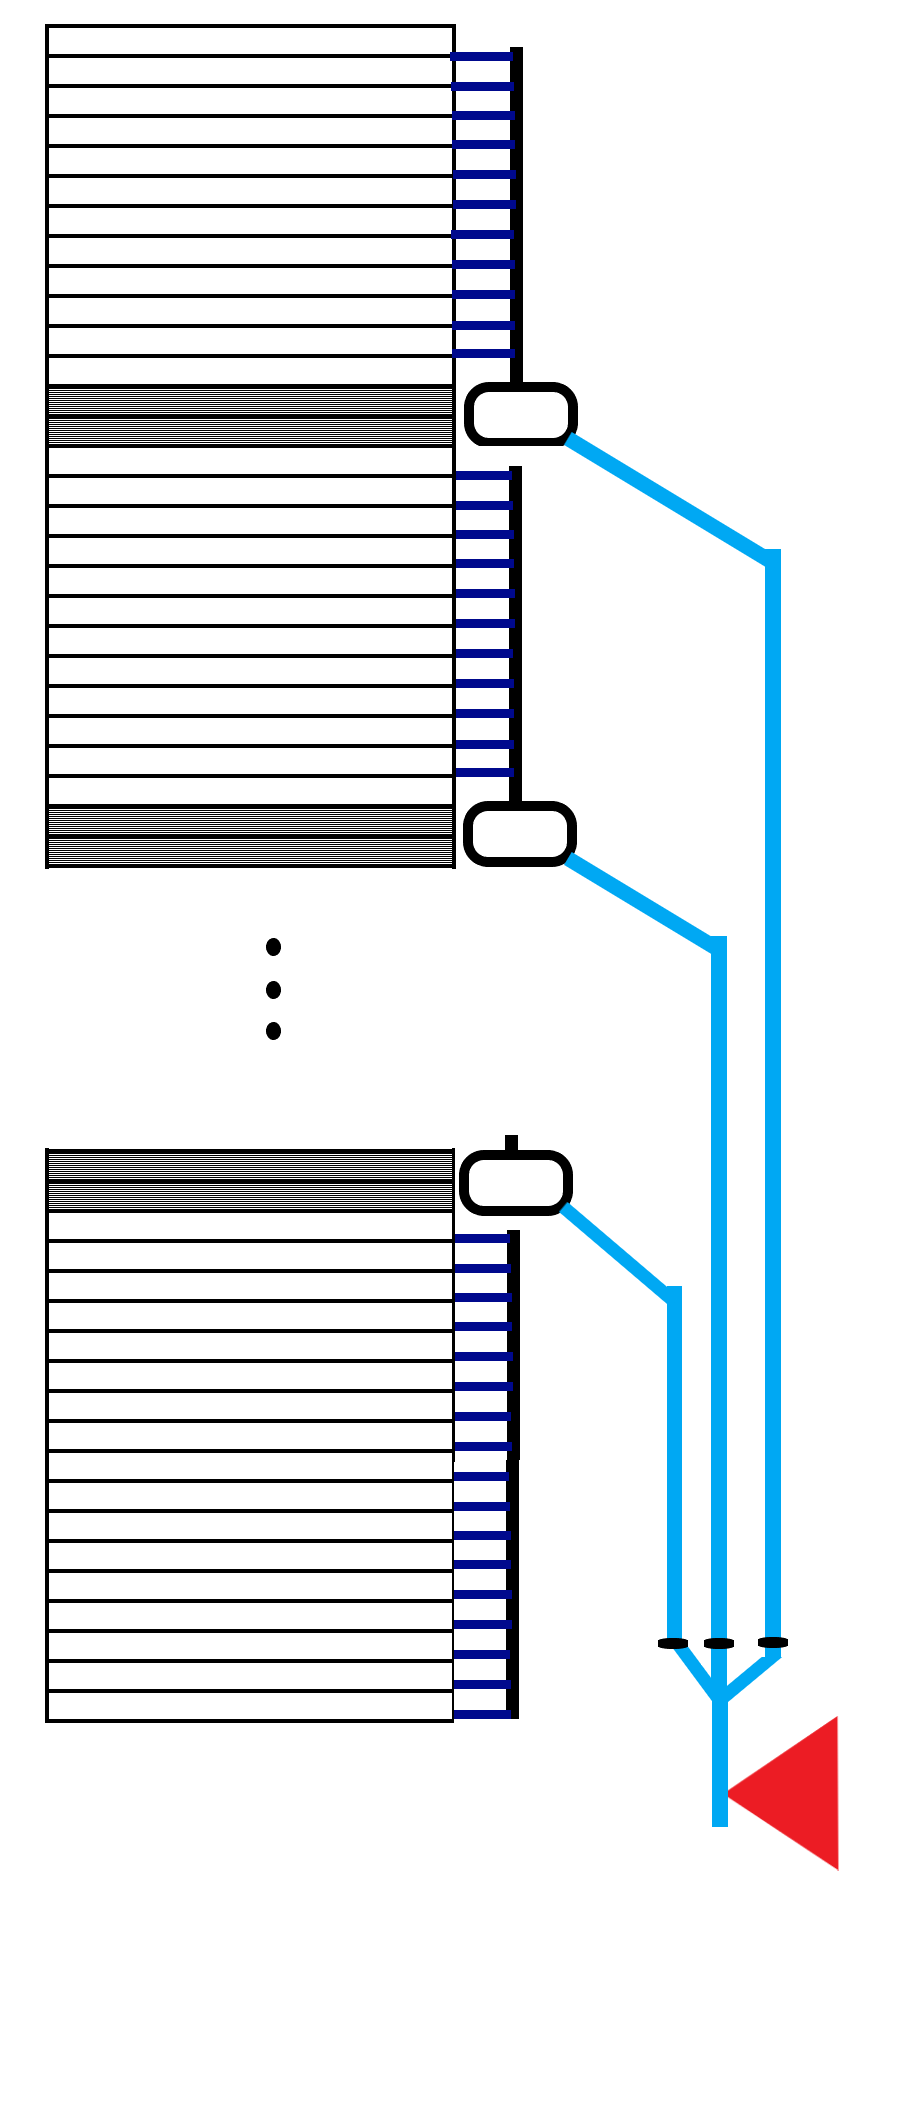
\includegraphics[width=7cm]{PrinzipGrobkonzept2.png}
	\caption{Prinzip Grobkonzep 2}
	\label{fig:PrinzipGrobkonzept2}
\end{figure}

Mit diesem Konzept wird ingesamt 44.59\si{kWh} pro Tag gewonnen, dies entspricht bei Stromkosten von 20\si{rp} einem Wert von 8.92\si{Fr}. Die Leistungsberechnungen sind im Anhang \ref{fig:BerechnungGrobkonzept2} \nameref{fig:BerechnungGrobkonzept2} zu finden.

\newpage

\paragraph{Grobkonzept 3}

Im Grobkonzept 3 wird die Geschwindigkeit des Abwassers ausgenutzt. Auch hier werden Druckleitungen eingebaut, um den Luftwiderstand zu eliminieren. So kann eine grössere Geschwindigkeit erreicht werden. In den unbenutzen Etagen wird das Wasser gesammelt und mit einer Druckleitung bis zur Turbine vor dem nächsten Tank geführt. Dies ist in der Abbildung \ref{fig:PrinzipGrobkonzept3} \nameref{fig:PrinzipGrobkonzept3} ersichtlich. 

\begin{figure} [H]
	\centering
	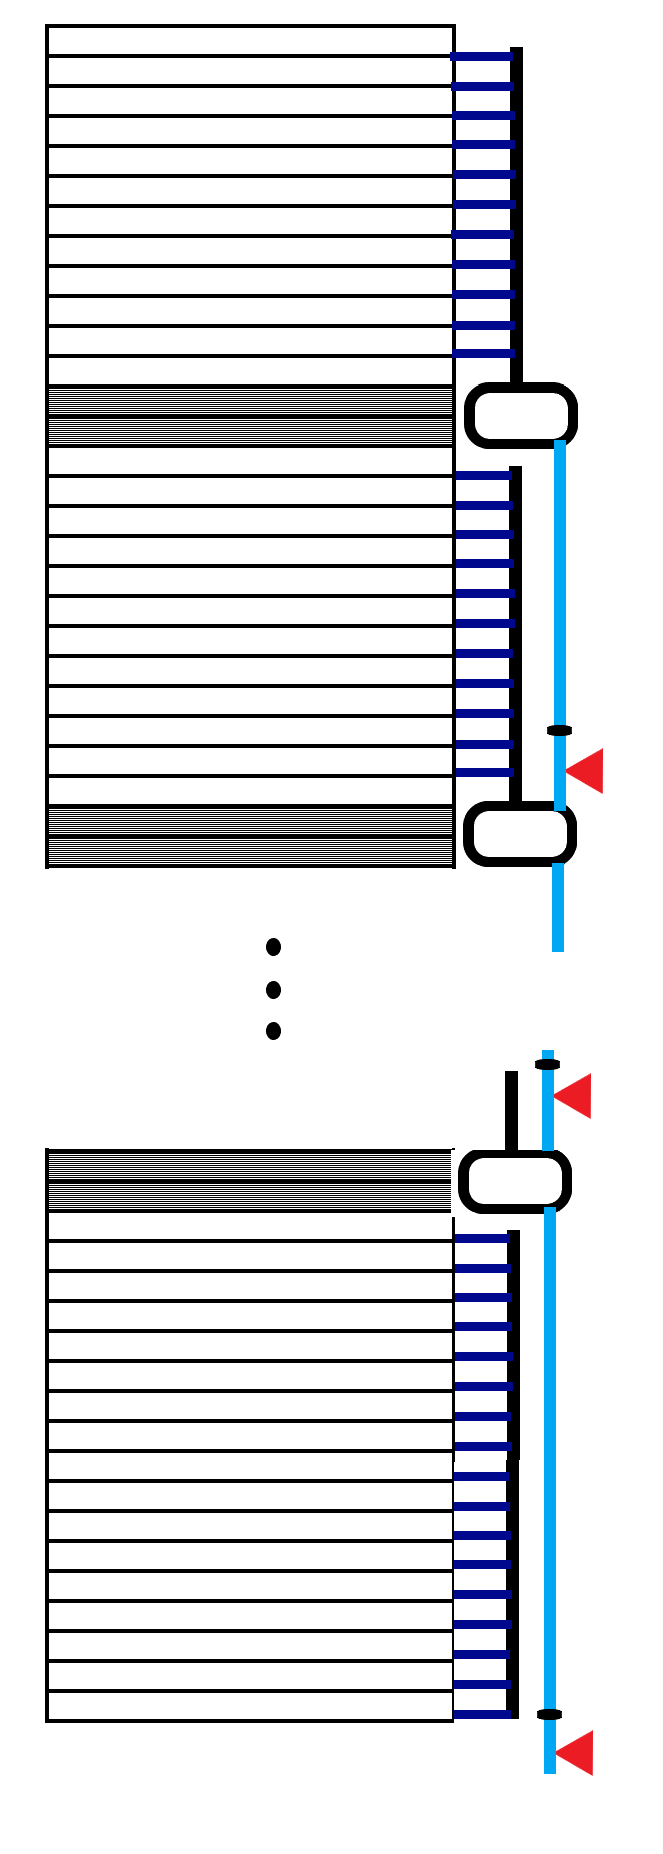
\includegraphics[width=6cm]{PrinzipGrobkonzept3.png}
	\caption{Prinzip Grobkonzep 3}
	\label{fig:PrinzipGrobkonzept3}
\end{figure}

Mit diesem Konzept wird ingesamt 42.62\si{kWh} pro Tag gewonnen, dies entspricht bei Stromkosten von 20\si{rp} einem Wert von 8.53\si{Fr}. Die Leistungsberechnungen sind im Anhang \ref{fig:BerechnungGrobkonzept3} \nameref{fig:BerechnungGrobkonzept3} zu finden.

\newpage

\paragraph{Grobkonzept 4}

Im Grobkonzept 4 wird die potenzielle Energie des Abwassers ausgenutzt. Damit die Wasserlifte nicht zu lang werden, werden diese Blockweise verbaut. Dies ist in der Abbildung \ref{fig:PrinzipGrobkonzept4} \nameref{fig:PrinzipGrobkonzept4} ersichtlich. Die obersten 5 Abschnitte bestehen aus 12 bewohnten und 2 ungenutzten Etagen. Der unterste Block besteht aus 16 bewohnten Etagen. Somit haben 5 Lifte eine Länge von 66.08\si{m} und der unterste Lift eine Länge von 80.24\si{m}

\begin{figure} [H]
	\centering
	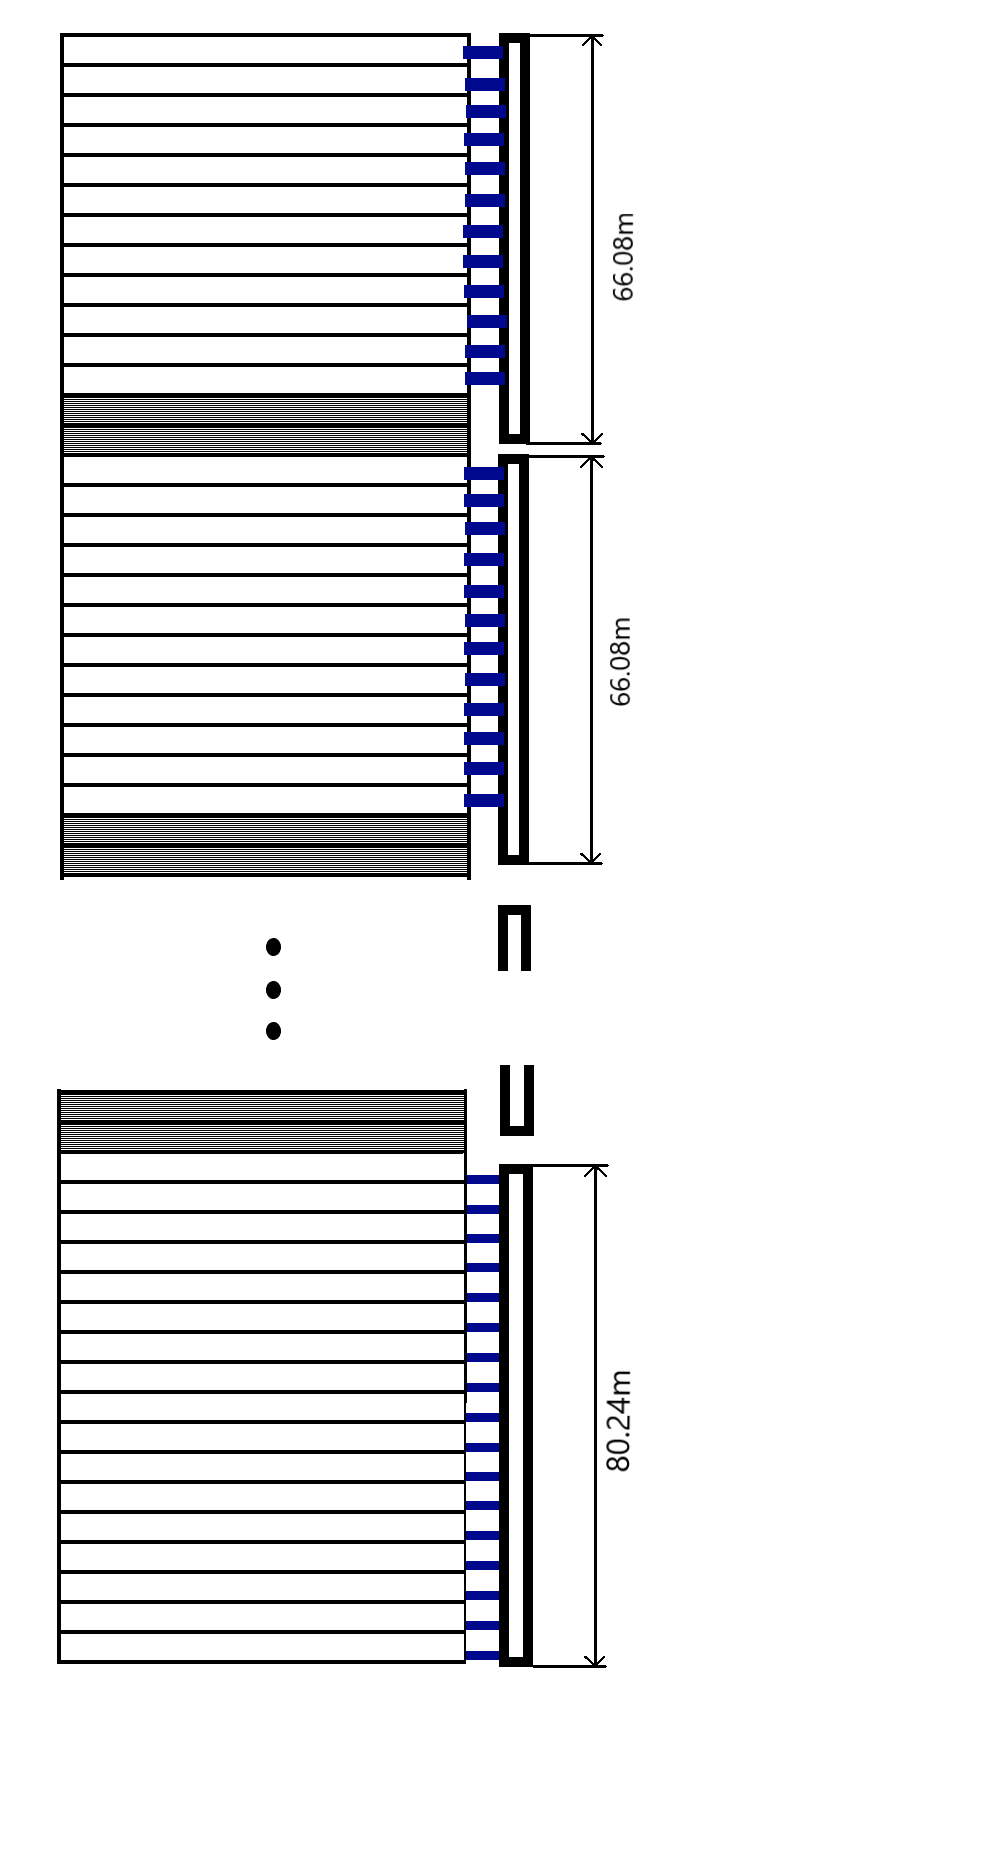
\includegraphics[width=8cm]{PrinzipGrobkonzept4.png}
	\caption{Prinzip Grobkonzep 4}
	\label{fig:PrinzipGrobkonzept4}
\end{figure}

Mit diesem Konzept wird ingesamt 53.08\si{kWh} pro Tag gewonnen, dies entspricht bei Stromkosten von 20\si{rp} einem Wert von 10.62\si{Fr}. Die Leistungsberechnungen sind im Anhang \ref{fig:BerechnungGrobkonzept4} \nameref{fig:BerechnungGrobkonzept4} zu finden.

\newpage
\subsection{Nutzwertanalyse} \label{subsec:nutzwertanlyse}
\renewcommand{\arraystretch}{1.5}
\newcommand{\vtcl}[1]{\rotatebox{90}{#1}}%\newcommand{\vtcl}[1]{\rotatebox{90}{\textbf{#1}}}
%\newcommand{\diagL}[1]{\diagbox{\hspace{#1}}{\hspace{#1}}}
Das Team konnte durch folgende Nutzwertanalyse bestimmen, dass das Grobkonzept 4 am ehesten in Fage kommt.
%\begin{table}[H]
%\small
%\begin{tabular}{l|llll|rr}
%&\vtcl{1.1. Wirkungsgrad}&\vtcl{1.2. Leistung}&\vtcl{1.3. Komplexität}&\vtcl{2.1. Platzbedarf}&\vtcl{Total}&\vtcl{Prozent}\\%\vtcl{2.1. Verstopfungsgefahr}&\vtcl{2.2. Platzbedarf}&\vtcl{2.3. Wartung}&\vtcl{Total}&\vtcl{Prozent}\\
%\hline
%1.1. Wirkungsgrad		&\cellcolor{black}	&0.5					&0.5					&0.5					&2.		&13\%\\
%1.2. Leistung			&0.5					&\cellcolor{black}	&1					&1					&4.5		&30\%\\
%1.3. Komplexität			&0.5					&0					&\cellcolor{black}	&0					&1.0		&6.5\%\\
%2.1. Verstopfungsgefahr	&1					&0					&1					&\cellcolor{black}	&0					&1					&3		&20\%\\
%2.1. Platzbedarf			&0.5					&0					&1					&\cellcolor{black}	&3.5		&24\%\\
%2.3. Wartung			&0.5					&0					&0.5					&0					&0					&\cellcolor{black}	&1.0		&6.5\%\\
%\hline
%\multicolumn{7}{c}{}&\textbf{15}&\textbf{100}\%\\
%\end{tabular}
%\end{table}
%\begin{scriptsize}
%Zeile-Kriterium ist wichtiger als Spalten-Kriterium 1\\
%Zeile-Kriterium ist gleich wichtig wie Spalten-Kriteriium 0.5\\
%Zeile-Kriterum ist weniger wichtig wie Spalternkriterium 0\\
%\end{scriptsize}
\newcolumntype{C}[1]{>{\centering}p{#1}}


\renewcommand\arraystretch{1.5}
\newcolumntype{R}[1]{>{\HY\RaggedLeft}p{#1}}
\newcolumntype{L}[1]{>{\HY\RaggedRight}p{#1}}
\renewcommand{\vtcl}[1]{\rotatebox{90}{\textbf{#1}}}
\begin{table}[H]
\small
\rotatebox{90}{
%|R{1.2cm}R{0.4cm}R{0.8cm} \scriptsize
%|R{1cm}R{0.2cm}R{0.5cm} \tiny
\begin{tabular}{lrR{0.8cm}|rrr|rrr|rrr|rrr|}%|R{1cm}R{0.5cm}R{0.8cm}
&&Max&\multicolumn{3}{c}{Grobkonzept 1}&\multicolumn{3}{c}{Grobkonzept 2}&\multicolumn{3}{c}{Grobkonzept 3}&\multicolumn{3}{c}{Grobkonzept 4}\\
\textbf{Zielkriterium}&\vtcl{Gewichtung}&\vtcl{Nutzwert}&\vtcl{Wert}&\vtcl{Erfüllungsgrad}&\vtcl{Nutzwert}&\vtcl{Wert}&\vtcl{Erfüllungsgrad}&\vtcl{Nutzwert}&\vtcl{Wert}&\vtcl{Erfüllungsgrad}&\vtcl{Nutzwert}&\vtcl{Wert}&\vtcl{Erfüllungsgrad}&\vtcl{Nutzwert}\\
\hline
&&&&&&&&&&&&&&\\
\rowcolor{hellgrau}
\multicolumn{3}{l|}{\textbf{Elektrotechnik}}&\multicolumn{3}{r|}{}&\multicolumn{3}{r|}{}&\multicolumn{3}{r|}{}&\multicolumn{3}{r|}{}\\
%										%G1 Wert		%G1 Erf.		G1 Nutz			%G2 Wert		%G2 Erf.		G2 Nutz			%G3 Wert		%G3 Erf.		G2 Nutz			%G4 Wert		%G4 Erf.		G4 Nutz
1.1. Wirkungsgrad	&25\%		&1.25	&32\%		&1			&0.25			&67.2\%		&3			&0.75			&64.1\%		&3			&0.75			&80\%		&4			&1.00\\
1.2. Leistung		&30\%		&1.50	&21.5kWh		&1			&0.33			&44.6kWh		&2			&0.66			&42.6kWh		&2			&0.66			&53.1kWh		&4			&1.20\\
%&&&&&&&&&&&&&&\\
\rowcolor{hellgrau}
\multicolumn{3}{l|}{\textbf{Abwassertechnik}}&\multicolumn{3}{r|}{}&\multicolumn{3}{r|}{}&\multicolumn{3}{r|}{}&\multicolumn{3}{r|}{}\\
%Verstopfungssicherheit&20\%		&1.000	&mässig		&2			&0.40			&mässig		&2			&0.4	0			&mässig		&2			&0.40			&mittel		&3			&0.60\\
2.1. Platzbedarf		&25\%		&1.00	&mässig		&4			&1.00			&erhöht		&2			&0.50			&erhöht		&2			&0.50			&mässig		&4			&1.00\\
%Wartung				&6.5\%		&0.325	&5			&2			&0.26			&3			&2			&0.26			&1			&4			&0.20			&1			&4			&0.20\\
\rowcolor{hellgrau}
\multicolumn{3}{l|}{\textbf{Allgemein}}&\multicolumn{3}{r|}{}&\multicolumn{3}{r|}{}&\multicolumn{3}{r|}{}&\multicolumn{3}{r|}{}\\
3.1. Schlichtheit	&20\%		&1.00	&8			&4			&0.8	0			&14			&3			&0.60			&15			&3			&0.60			&10			&4			&0.80\\
&&&&&&&&&&&&&&\\
\hline
Summe				&100.0\%		&5.000	&			&			&2.38			&			&			&2.51			&			&			&2.51			&			&			&4.00\\
Erfüllungsgrad [\%]	&&100.0				&			&			&48				&			&			&50				&			&			&50				&			&			&80\\
\multicolumn{3}{l}{\textbf{Rangfolge}}&\multicolumn{3}{r|}{\textbf{3}}&\multicolumn{3}{r|}{\textbf{2}}&\multicolumn{3}{r|}{\textbf{2}}&\multicolumn{3}{r|}{\textbf{1}}\\
\multicolumn{15}{l}{\textbf{}}\\
\multicolumn{15}{l}{\textbf{}}\\
\end{tabular}
}
\rotatebox{90}{
\scriptsize
\begin{tabular}{lC{1.2cm}C{1.2cm}C{1.2cm}C{1.2cm}C{1.2cm}l}
\multicolumn{7}{c}{\textbf{Erfüllungsgrad}}\\
\hline
&min.&&mittel&&max.&\\
&\textbf{1}&\textbf{2}&\textbf{3}&\textbf{4}&\textbf{5}&Messgrösse\\
\hline
1.1. Wirkungsgrad				&<50&51-60&61-70&71-80&>81&\%\\
1.2. Leistung					&<40&40-44&45-50&51-54&>55&kWh\\
%2.1. Verstopfungssicherheit		&gering&mässig&mittel&erhöht&hoch&a)\\
2.1. Platzbedarf					&hoch&erhöht&mittel&mässig&gering&Schätzung m\textsuperscript{2}\\
%2.3. Wartung						&52-13&12-6&5-2&1&0&b)\\
3.1. Schlichtheit				&>20&20-16&15-11&10-6&1-5&Anz. versch. Teile\\
\end{tabular}
}
\caption{Nutzwertanalyse}\label{tab:nutzwertanalyse}
\end{table}

\section{Detailkonzept} \label{sec:detailkonzept}

Das Konzept mit den Wasserliften ist am besten geeignet für unsere Anwendung. Es existieren bereits «Rohrkettenförderer», aber diese werden ausschliesslich verwendet, um Produkte nach oben zu befördern. Wir nutzen dieses System, um das Abwasser nach unten zu befördern und dabei Energie zu gewinnen. Es werden insgesamt sechs Lifte benötigt. Fünf Lifte überwinden je 60.08\si{m} und der unterste Lift überwindet 80.24\si{m}. In der Abbildung \ref{fig:PrinzipGrobkonzept4} \nameref{fig:PrinzipGrobkonzept4} ist dies grafisch dargestellt.

\subsection{Elektronik}

\begin{figure}[H]
\centering
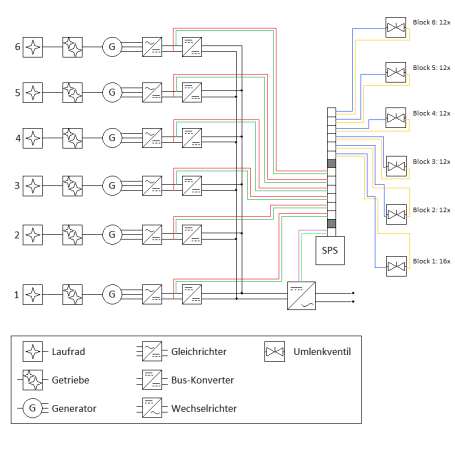
\includegraphics[width=14cm]{Skizze_GK4.png}
\caption{Prinzipschema}
\label{fig:Prinzipschema}
\end{figure}

Die potentielle Energie des Abwassers wird über ein Laufrad in kinetische Energie umgewandelt. Mit einem Getriebe wird die vom Laufrad kommende Drehzahl dem Generator angepasst, welcher die kinetische Energie in elektrische umwandelt. Der Gleichrichter transformiert den Dreiphasenwechselstrom in einen zweipoligen Gleichstrom. Anschliessend wird durch einen DC-DC Konverter eine Rückkoppelung auf den Genreator verhindert. Weiter stellt der Konverter sicher, dass eine stabile Ausgangsspannung anliegt und der DC-Bus galvanisch vom Generator und vom Wechselrichter getrennt ist. Die summierte Energie aller sechs Generatorenstränge wird über einen Wechselrichter ins Stromnetz eingespeist. Zur Überwachung und auch zur Ansteuerung der Umlenkventile wird eine SPS verwendet.

\bigskip

\paragraph{Generator} \label{para:generator}

Der Wasserverbrauch und somit die Abwasserproduktion im Hochhaus ist nicht über den ganzen Tag konstant. Für die Dimensionierung der Bauteile ist es aber wichtig, den Spitzenwert der Abwasserproduktion zu kennen. Dieser kann aus Abbildung \ref{fig:tagesGangKurve} ausgelesen werden und liegt zwischen 7 und 8 Uhr morgens. Während dieser Stunde fliesst etwa 15\% des Abwassers ab, also müssen alle Komponenten auf diese Spitzenbelastung ausgelegt sein. 
Der unterste Lift ist am längsten und befördert gleichzeitig die gesamte Abwassermenge. Es wurde berechnet, dass er pro Tag \(70.22 MJ\) potentielle Energie aufnimmt. Mit einem Wirkungsgrad von 80\% des Liftes ergibt das 56.3 MJ, die der Generator umsetzten muss, \(15\%\) oder \(8.4 MJ\) dieser Energie zwischen 7 und 8 Uhr morgens. Der Generator muss also eine Mindestleitung von \(8.4 MJ / 3600 s = 2333 W \) aufweisen. Da die Abwassermenge auch während dieser Stunde nicht ganz konstant ist und zeitweise höher sein könnte, sollte der Generator eine Mindestleitung von \(3 kW\) haben.

\begin{figure}[H]
\centering
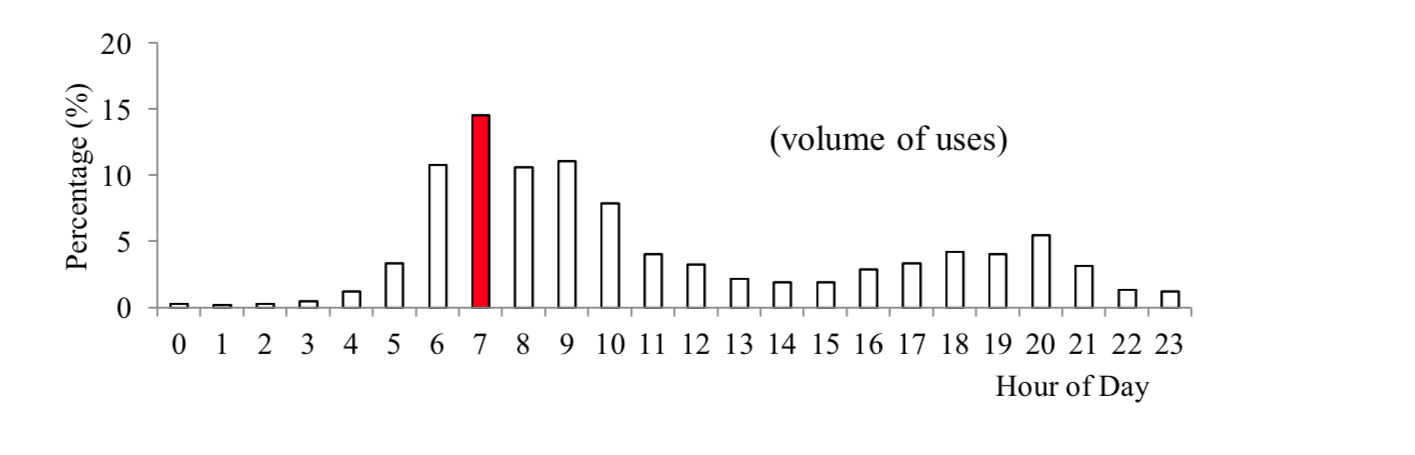
\includegraphics[width=\linewidth]{tagesGangKurve.png}
\caption{Typische Tagesgangkurve. \cite{peakWaterDemand}}
\label{fig:tagesGangKurve}
\end{figure}

Aufgrund dieser Berechnungen haben wir uns für einen Eastern Lion STC-3 Dreiphasengenerator entschieden (Siehe Abbildung \ref{fig:Generator}).  

\begin{figure}[H]
\centering
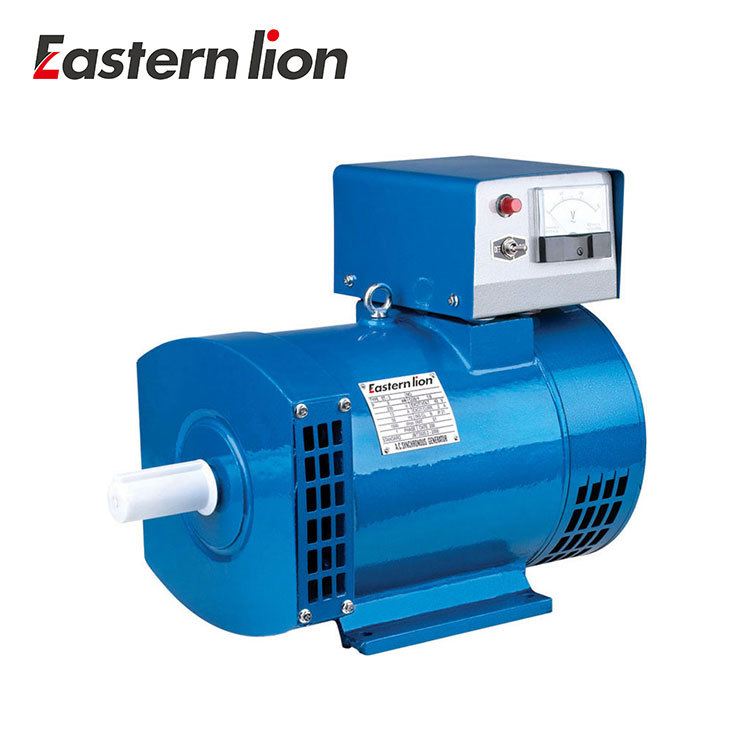
\includegraphics[width=6cm]{Generator.jpg}
\caption{Eastern Lion STC-3 \cite{generator}}
\label{fig:Generator}
\end{figure}

Dieser Generator ist mit einem Preis von 110\$ sehr günstig und erfüllt mit einer Leistung von 3 kW unsere Anforderungen.
\begin{table}[H]
\small
\begin{center}
\begin{tabular}{ll}
\hline
\textbf{Anforderung}&\textbf{Wert}\\
\hline
Leistung&\(3kW\)\\
Ausgang&	3 Phasen \(380V/120V\)\\
Drehzahl&1500 bis \(1800 U/min\)\\
Wirkungsgrad&92\%\\
Kosten&110CHF\\
\end{tabular}
\caption{Anforderungen an den Generator}
\end{center}
\end{table}


\paragraph{Gleichrichtung nach Generator}

Die dreiphasige Wechselspannung des Generators wird mit einem Gleichrichter in Gleichspannung umgewandelt. Wir haben uns für einen SETEC SET4850 Gleichrichter entschieden (siehe Abbildung \ref{fig:Gleichrichter}). Dieser besteht nicht nur aus einem Dreiphasen-Gleichrichter, sondern ist auch ein Netzteil, das unter anderem einen geregelten \(48Vdc\) Ausgang hat. Dieser Ausgang kann somit direkt über den DC Bus mit den Wechselrichtern der anderen Turbinen parallel geschaltet werden. Gesteuert und überwacht wird das Gerät über einen RS 485 Bus.

\begin{figure}[H]
\centering
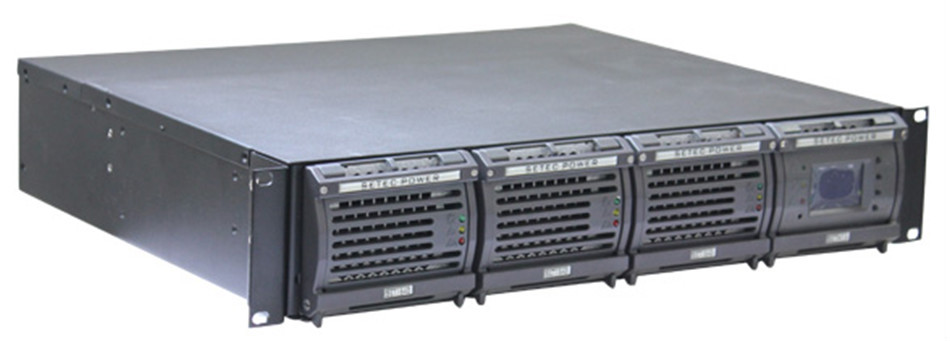
\includegraphics[width=6cm]{Gleichrichter.jpg}
\caption{Setec SET4850 \cite{gleichrichter}}
\label{fig:Gleichrichter}
\end{figure}

\begin{table}[H]
\small
\begin{center}
\begin{tabular}{ll}
\hline
\textbf{Anforderung}&\textbf{Wert}\\
\hline
Leistung&\(3 kW\)\\
Eingang&AC \(3 * 380V\)\\
Ausgang&DC \(48V/110V/220V\)\\
Genauigkeit&\(\pm 0.5 \%\)\\
Wirkungsgrad&\(96\%\)\\
Steuerung&RS 485\\
Kosten&300CHF\\
\hline
\end{tabular}
\caption{Anforderungen an den Gleichrichter}
\end{center}
\end{table}


%http://www.farnell.com/datasheets/2333819.pdf?_ga=2.222713307.1750103157.1543910091-374399726.1543659672

\paragraph{Wechselrichter für Netzeinspeisung} \label{par:WechselrichterNetz}

Damit die gewonnen Leistung in das Netz eingespiesen werden kann, muss der Wechselrichter folgende Eigenschaften aufweisen. 

\begin{table}[H]
\small
\begin{center}
\begin{tabular}{ll}
\hline
\textbf{Anforderung}&\textbf{Wert}\\
\hline
Leistung&\(9 kW\)\\
Ausgang&3 Phasen\\
Kosten&<4000CHF\\
\hline
\end{tabular}
\caption{Anforderungen an den Wechselrichter}
\end{center}
\end{table}

In der Förderungsanlage wird ein Asynchrongenerator verbaut. Die Firma Voltacon ist bekannt für ihre Hochleistungswechselrichter.

Das Modell Hybrid Wechselrichter HSI10000 entspricht den gewünschten Anforderungen für unsere Förderungsanlage. Der Wechselrichter transformiert die 48VDC auf 230VAC mit einer Frequenz von 50\si{\hertz}. Das Gerät kann bis zu einer Leistung von 10KW erbringen. Mittels integrierten Displays kann die erbrachte Leistung zusätzlich abgelesen werden. 


\begin{figure} [H]
	\centering
	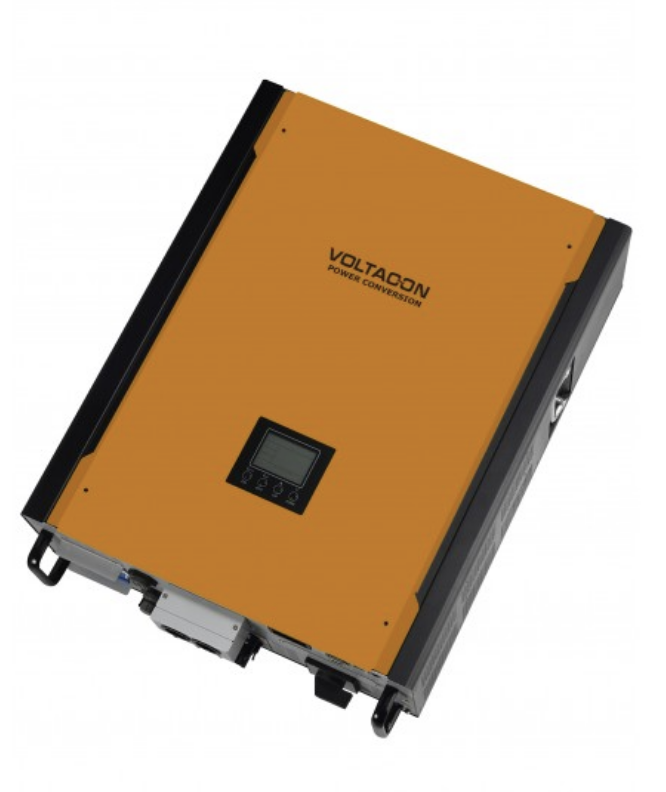
\includegraphics[width=10cm]{Voltacon.png}
	\caption{Wechselrichter \cite{Voltaconsolar}}
	\label{fig:Wechselrichter}
\end{figure}

Gemäss Datenblatt lassen sich Ströme bis 200A regeln. Der Wechselrichter hat einen netzunabhängigen Energiespeicher (Batterie-Backup). Um die Daten des Wechselrichters weiterzuleiten stehen verschieden Kommunikationsmittel zur Verfügung. Die Informationen können über einen USB Port, RS-232 oder den SNMP (Simple Network Management Protocol) Überwachungssoftware für Echtzeitstatusanzeige und -steuerung übermittelt werden. Die Kosten des Wechselrichters belaufen sich auf 3'401\si{Fr}.

\newpage


\paragraph{Kontrollsystem}

Das Kontrollsystem steuert und überwacht die Anlage und ist wie folgt aufgebaut: Auf einem PC ist eine C\# Software installiert. Das Programm kommuniziert über ModbusTPC mit der SPS und kann die Anlage so steuern. In der Abbildung \ref{fig:beckhoff} \nameref{fig:beckhoff} ist die SPS von Beckhoff ersichtlich.

\bigskip

\begin{figure} [H]
	\centering
	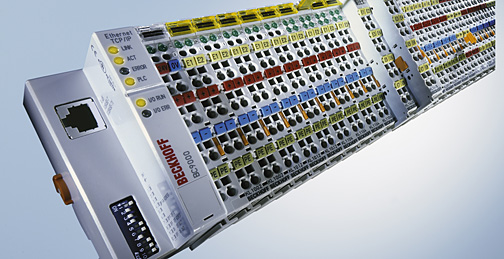
\includegraphics[width=10cm]{Beckhoff.jpg}
	\caption{SPS von Beckhoff \cite{beckhoff}}
	\label{fig:beckhoff}
\end{figure}

In der Software kann über eine grafische Oberfläche ein Benutzer einfach auf die Anlage zugreifen, steuern und Informationen ablesen. Das Programm hat zwei verschiedene Modi. Einen manuellen Modus und einen Betriebsmodus. Im manuellen Modus kann der Betrieb der Anlage für Wartungsarbeiten angepasst werden. So können die Ventile einzeln oder blockweise geschaltet werden. Im Betriebsmodus werden nur im Störungsfall die Ventile automatisch geschalten, um die Sicherheit zu gewährleisten. Wenn möglich werden nur einzelne Blöcke deaktiviert, damit die Anlage weiterhin Strom produzieren kann. In beiden Modi wird die Stromgewinnung überwacht. So wird angezeigt, welcher Generator gerade wie viel Strom erzeugt. Der Wechselrichter, der unter Wechselrichter für Netzeinspeisung beschrieben ist, kann über einem USB-Port eine serielle Kommunikation mit dem PC aufbauen. Das Programm kann die Informationen der aktuellen Energiegewinnung über diese Schnittstelle auslesen, speichert diese in einem Log. File und gibt diese an die Benutzeroberfläche weiter. Die gesammelten Daten können im Programm ausgewertet und grafisch dargestellt werden. Für dieses Kontrollsystem werden folgende Komponenten benötigt.

\bigskip

\begin{table}[H]
\small
\begin{tabular}{lllrr}
\hline
\textbf{Anzahl}&\textbf {Komponente}&\textbf{Bezeichnung}&\textbf{Stückpreis [\si{CHF}]}&\textbf{Gesamtpreis [\si{CHF}]}\\
\hline
1&Kontrollklemme&BK9050&200&200\\
20&Digitale Ausgangsklemme&KL1114&100&2000\\
20&Digitale Eingangsklemme&KL2134&100&2000\\
7& Analoge Eingangsklemme&KL2134&100&700\\
1&PC&Dell&1000&1000\\
\hline
\end{tabular}
\caption{Kostentabelle für Kontrollsystem}
\end{table}

\bigskip

Die Kosten für die Komponenten betragen 5900 \si{Fr} \cite{beckhoff}. Für die Entwicklung der Software werden 3 PM benötigt, was einmalig 48'000\si{Fr} kostet. 



\newpage


\subsection{Mechanik}

\paragraph{Rohrkette}

In der Industrie werden Rohrkettenförderer für den Transport von Schuttgüter verwendet. In der Abbildung \ref{fig:Rohrkettenfoerderer} \nameref{fig:Rohrkettenfoerderer} ist der Innenaufbau eines solchen Rohrkettenförderers ersichtlich.

\begin{figure} [H]
	\centering
	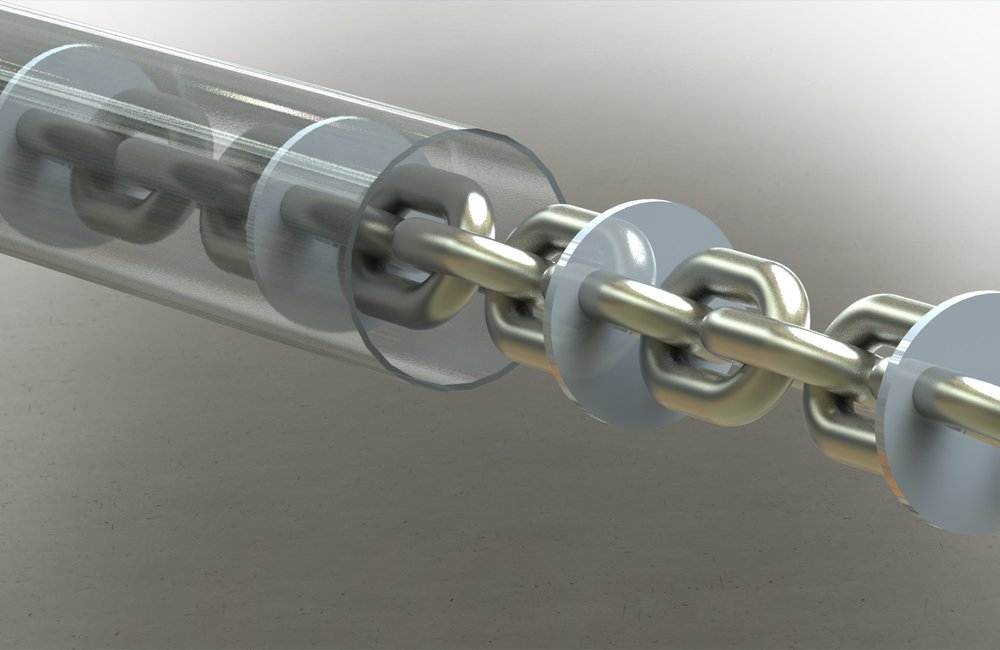
\includegraphics[width=6cm]{Rohrkettenfoerderer.jpg}
	\caption{Innenaufbau Rohrkettenförderer \cite{abconvey}}
	\label{fig:Rohrkettenfoerderer}
\end{figure}

Wir wollen keinen Schutt nach oben befördern, daher muss dieses System auf unsere Anforderungen angepasst werden. Diese Anforderungen sind, dass die verwendeten Materialien Robust gegenüber Korrosion sind, da das Abwasser aggressiv auf diese wirkt. Weiter müssen, um einen möglichst hohen Wirkungsgrad zu erreichen, die Platten mit möglichst kleinem Spielraum zur Aussenwand konstruiert werden, damit das Wasser nicht einfach auf der Seite herunterfliessen kann und gleichzeitig nicht eine zu grosse Reibung erzeugt wird. Die Drehachse, an dem der Generator angeschlossen wird, ist ein Stösselkettenrad. Dieses ist in der Abbildung \ref{fig:stoesselkettenrad} \nameref{fig:stoesselkettenrad} zu sehen

\begin{figure} [H]
	\centering
	\includegraphics[width=6cm]{Stoesselkettenrad.jpg}
	\caption{Stösselkettenrad \cite{schrage}}
	\label{fig:stoesselkettenrad}
\end{figure}


Um diesen Wasserlift zu bauen, beauftragen wir die Firma Schrage, ein führender Speziallist für Rohrketten, die in Deutschland zu Hause ist. Die Kosten belaufen sich für die 60.08\si{m} Höhendifferenz auf ca. 10'000\si{Fr} pro Lift und für die 80.24\si{m} Höhendifferenz auf ca. 13'000\si{Fr}. Insgesamt würde die Analage mit den Rohrketten, Rohr und Stösselkettenrad ca. 63'000\si{Fr} kosten. \cite{schrage}

\newpage

\paragraph{Getriebe}
Da der Generator eine viel höhere Drehzahl benötigt, als dass der Lift zur Verfügung stellt, muss ein Getriebe verwendet werden. Doch um dieses zu dimensionieren, muss man zuerst wissen, wie schnell sich der Wasserlift überhaupt bewegt. Dies ist abhängig von der Wassermenge und vom Rohrdurchmesser. Das Modellhochhaus hat 76 bewohnte Stockwerke mit je fünf Bewohnern, die durchschnittlich 314 Liter Wasser am Tag verbrauchen. Die Gesamtwassermenge beträgt also \(76 * 5 * 314 = 119320 l/24h\), die vollständig durch den untersten Wasserlift abfliesst. Anhand der Tagesgangkurve (siehe Abbildung \ref{fig:tagesGangKurve}) kann man ablesen, dass 15\% des Abwassers zwischen 7 und 8 Uhr morgens abgelassen wird. Dies entspricht einer Abwassermenge von \(119320 * 0.15 = 17898 l\), etwa \(18 m^3 \), die innerhalb einer Stunde durch den untersten Wasserlift muss. Aus den Tabellen zu den Fördermengen von Schrage (Siehe Abbildung \ref{fig:foerdermengen}) kann man nun ablesen, bei welchem Rohrdurchmesser welche Geschwindigkeit nötig ist, um diese 18 Kubikmeter Abwasser zu befördern. 

\begin{figure} [H]
	\centering
	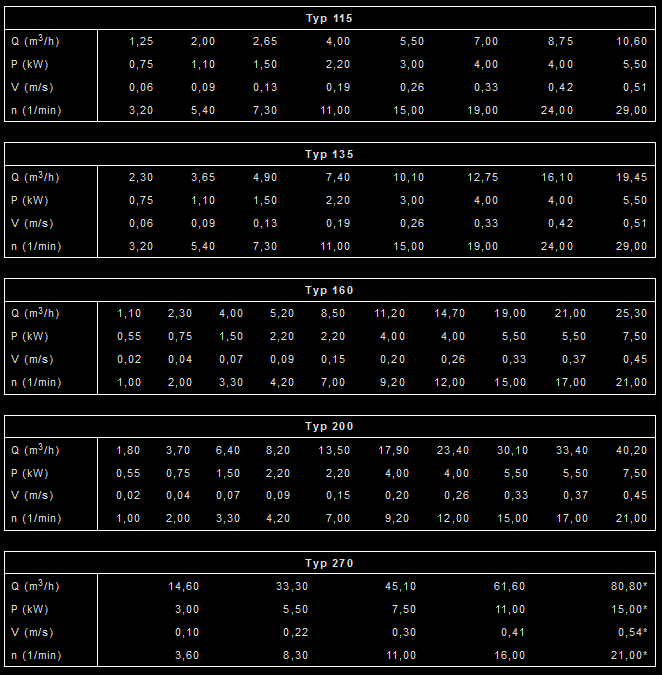
\includegraphics[width=12cm]{Foerdermengen.PNG}
	\caption{Fördermengen \cite{schrage}}
	\label{fig:foerdermengen}
\end{figure}

Um etwas Reserve zu haben, falls einmal eine grössere Abwasserspitze auftritt, sollte das Rohr einen Durchmesser von mindestens \(160mm\) haben. Bei \(18 m^3 /h \) und einem Rohrdurchmesser von \(160mm\) hat die Förderkette also eine Geschwindigkeit von etwa \(0.3 m/s \). Bei diesem Rohrdurchmesser hat das Stösselkettenrad einen Durchmesser von etwa \(400mm\)\cite{schrage} und einen Umfang von \(400mm * \pi = 1257mm = 1.257m\). Somit hat das Stösselkettenrad eine Drehzahl von \(1.257m * 0.3 m/s * 60s = 22,6 U/min\). Aufgrund der kleinen Drehzahl aber relativ grossen Leistung von maximal \(2300 W\) hat der Wasserlift ein relativ hohes Drehmoment von \( 2300 /(2 * \pi * 22.6/ 60) = 972 N/m\). Der Generator hat eine maximale Drehzahl von \(1800 U/min\), braucht aber nur wenig Drehmoment. Das Getriebe muss also die Drehzahl des Liftes erhöhen, dabei ist das nötige Übersetzungsverhältnis etwa 1:80. 
\begin{table}
\small
\begin{center}
\begin{tabular}{ll}
\hline
\textbf{Anforderung}&\textbf{Wert}\\
\hline			
Übersetzungsverhältnis&1:80\\
Leistung&$\geq$\(3 kW\)\\		
Eingangsdrehzahl&\(22.6 U/min\)\\
Eingangsdrehmoment&$\geq$\(1000 Nm\)\\	
Ausgangsdrehzahl&\(1800 U/min\)\\
Ausgangsdrehmoment&$\geq$\(20 Nm\)\\
\hline
\end{tabular}
\caption{Anforderungen an das Getriebe}
\end{center}
\end{table}
Es wurden Anfragen an mehrere mögliche Hersteller gesendet, allerdings bislang ohne Antwort. Wir schätzen den Preis pro Getriebe auf 1000.- Franken, also insgesamt ~6000.- Franken.

\paragraph{Umleitventil}

Da wir für Störungsfälle eine Fallleitung eingeplant haben, muss in jeder Etage ein Umleitungsventil installiert werden. Das Modell 167 PVC-U von GF Piping Systems, das in der Grafik \ref{fig:Umleitungsventil} zu sehen ist, ist optimal für diese Bedingung geeignet. Die integrierte Steuerung kann von einer Spannung von 24V angesteuert werden. Somit können wir es im SPS System integrieren. Pro Umleitventil rechnen wir mit 100CHF.

 \begin{figure} [H]
	\centering
	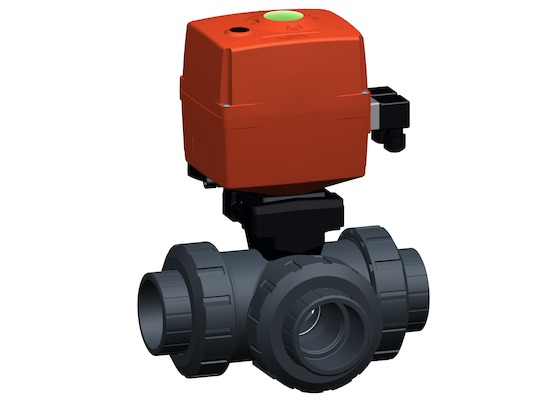
\includegraphics[width=6cm]{umleitVentil.jpg}
	\caption{Ventil \cite{Umleitungsventil}}%TODO MICHEL link in bibtex einfuegen https://www.gfps.com/appgate/ecat/common_flow/10006F/CH/de/109564/721624/721636/P420683/product.html
	\label{fig:Umleitungsventil}
\end{figure}

%TODO Frank: Alle Kosten zusammentragen
\section{Wirtschaftlichkeit} \label{sec:wirtschaftlichkeit}
In diesem Abschnitt berechnen wir anhand grober Schätzungen die Wirtschaftlichkeit unseres Systems. 
Als Indikator für die Wirtschaftlichkeit wird die Amortisationszeit verwendet.
\subsection{Annahmen}
Für die vereinfachung der Amortisationsrechnung wurden folgende Annahmen getroffen:\\
\begin{itemize}  
\item Das Hochhaus wird neu gebaut, deshalb entstehen keine Umbaukosten.
\item Als Investitionskosten zählen wir die Einbaukosten der zusätzlichen Infrastruktur, die Materialkosten und die Entwicklungskosten.
\item Pro Jahr entsteht ein Service- und Reperaturaufwand in der Höhe von schätzungsweise 1'000 CHF.
\item Die Einbaukosten der zusätzlichen Infrastruktur betragen etwa 10'000 CHF.
\item Es steht keine Wohnung leer.
\item Der Wasserverbrauch ist konstant.
\end{itemize}

\renewcommand\arraystretch{1.2}
\newcolumntype{Z}[1]{>{\HY\RaggedLeft\bfseries}p{#1}}
\subsection{Kosten}
\begin{table}[H]
\small
\begin{tabular}{L{4cm}R{1.5cm}rR{2cm}Z{2cm}}
%\multicolumn{4}{l}{\textbf{Investitionskosten}}\\
\hline
\textbf{Kostenkategorie}&\textbf{Anzahl}&\textbf{Preis[CHF]/Element}&\textbf{Preis[CHF]}&\\
\hline
\rowcolor{hellgrau}
\multicolumn{4}{l}{\textbf{Einbaukosten}}&10'000\T\\
Einbau zus. Infrastruktur&1&10'000&10'000&\B\\
\rowcolor{hellgrau}
\multicolumn{4}{l}{\textbf{Materialkosten}}&88'160\T\\
\multicolumn{4}{l}{\textit{Mechanik}}&\normalfont{69'000}\\
Rohrkette 60.08m&5&10'000&50'000&\\
Rohrkette 80.24m&1&13'000&13'000&\\
Getriebe&6&1000&6'000&\\
\multicolumn{4}{l}{\textit{Elektrotechnik}}&\normalfont{11'760}\T\\
Generator&6&110&660&\\
Gleichrichter&6&300&1'800&\\
Wechselrichter&1&3'401&3'401&\\
Kontrollsystem&1&5900&5900&\\
\multicolumn{4}{l}{\textit{Abwassertechnik}}&\normalfont{7'400}\T\\
Umleitventil&74&100&7'400&\B\\
\rowcolor{hellgrau}
\multicolumn{4}{l}{\textbf{Entwicklungskosten}}&48'000\T\\
Software&1&48'000&48'000\B\\
\hline
%\rowcolor{grau}
\multicolumn{3}{l}{\textbf{Gesamt}}&&146'160\T\\
&&&\\
&&&\\
\end{tabular}
\caption{Kostentabelle}\label{tab:kostentabelle}
\end{table}
\newpage
\subsection{Amortisationszeit}
Mit der Formel $A = \tfrac{K}{R}$ wird nun die Amortisationszeit (A) berechnet, wobei K die einmaligen Investitionskosten sind, die man aus der Tabelle \ref{tab:kostentabelle} entnehmen kann. R ist der jährliche Rückfluss, also in unserem Fall der Ertrag aus dem Stromgewinn abzüglich des Service- und Reperaturaufwands.\\

\bigskip
K = 146'160 CHF

\bigskip
R = 365$\tfrac{T}{J}\cdot$10.62$\tfrac{CHF}{T}$ - 1'000$\tfrac{CHF}{J}$ = 2'876$\tfrac{CHF}{J}$

\bigskip
$A = \tfrac{146'160CHF}{2'876 \tfrac{CHF}{J}} =$ 50.82$J$

\bigskip
Trotz Verwendung optimistisch geschätzter Werte braucht es 51 Jahre, bis die Investitionskosten amortisiert sind. In der Regel sind z.B. Solaranlagen nach 9-15 Jahren amortisiert bei einer Lebensdauer von 30 Jahren \cite{helion}. Für unser System wären 10-15 Jahre Amortisationszeit wünschenswert gewesen, aber nicht realisierbar.
Angenommen das System würde ein zweites Mal eingebaut, könnten die Entwicklungskosten für die Software, also 48'000 CHF, gespart werden. Aber auch dann wäre das System erst nach 30 Jahren amortisiert. Unser System ist also unwirtschaftlich.
\section{Projektvereinbarung} \label{sec:projektvereinbarung}
\begin{tabular}{l l}
\textbf{Auftraggeber} &\\
&\\
Dr. Luca Dalessandro \\
&\\
&\\
&\\
\rule{6cm}{0.5pt} & \rule{6cm}{0.5pt}\\
Ort, Datum & Unterschrift\\
&\\
&\\
&\\
&\\
&\\
&\\
\textbf{Projektleiter} &\\
&\\
Niklaus Schwegler&\\
&\\
&\\
&\\
\rule{6cm}{0.5pt} & \rule{6cm}{0.5pt}\\
Ort, Datum & Unterschrift\\
\end{tabular}



%%---BIBLIOGRAPHY------------------------------------------------------------------------

{\sloppypar
\selectlanguage{english}	
\setlength{\bibitemsep}{\baselineskip}
\printbibliography[heading=bibintoc]
\label{sec:lit}
}

%%---Anhang------------------------------------------------------------------------

\section{Anhang} \label{sec:anhang}



\subsection{Testkonzept} \label{subsec:eltech}
\begin{figure}[H]
	\centering
	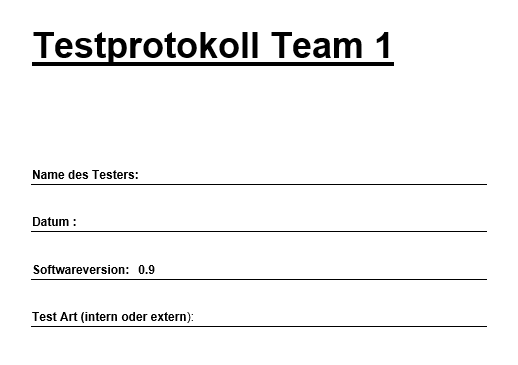
\includegraphics[width=16cm]{Protokoll.png}
	\label{fig:Protokoll}
\end{figure}

\begin{figure}[H]
	\centering
	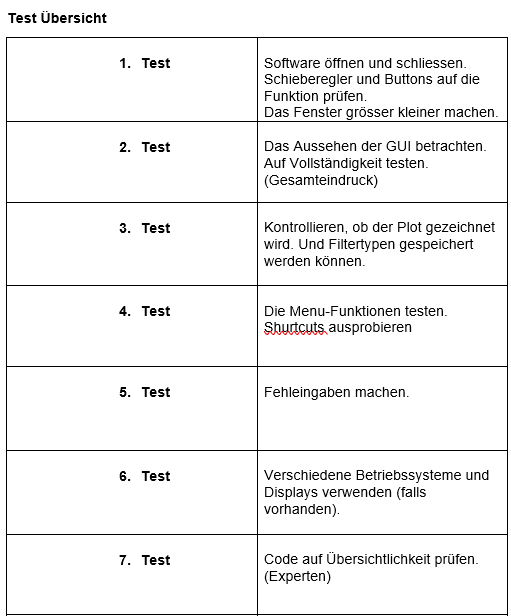
\includegraphics[width=16cm]{uebersicht.png}
	\label{fig:übersicht}
\end{figure}

\begin{figure}[H]
	\centering
	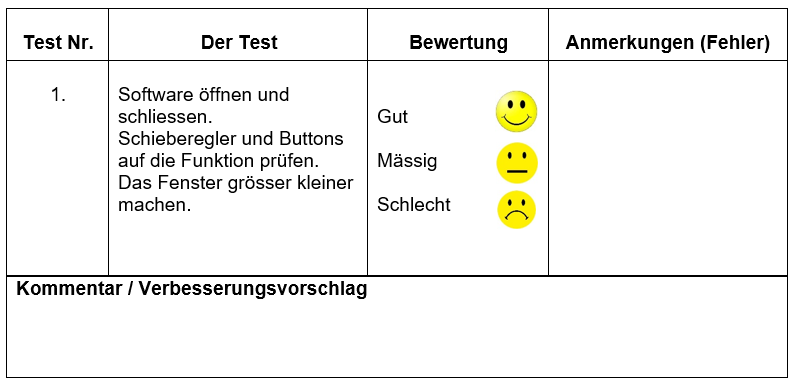
\includegraphics[width=16cm]{Test1.png}
	\label{fig:Test1}
\end{figure}

\begin{figure}[H]
	\centering
	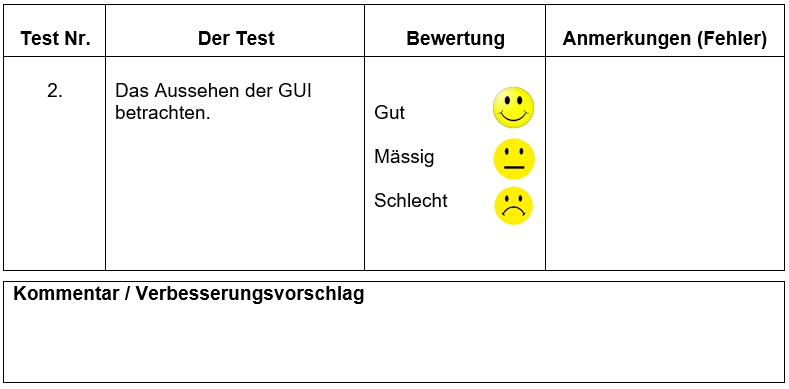
\includegraphics[width=16cm]{Test2.png}
	\label{fig:Test2}
\end{figure}

\begin{figure}[H]
	\centering
	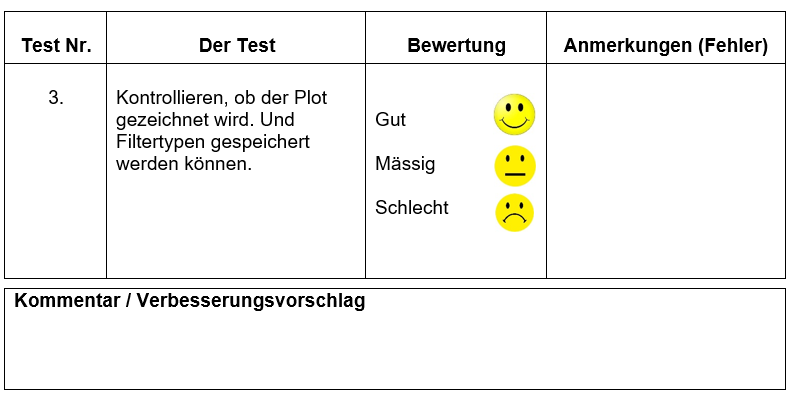
\includegraphics[width=16cm]{Test3.png}
	\label{fig:Test3}
\end{figure}

\begin{figure}[H]
	\centering
	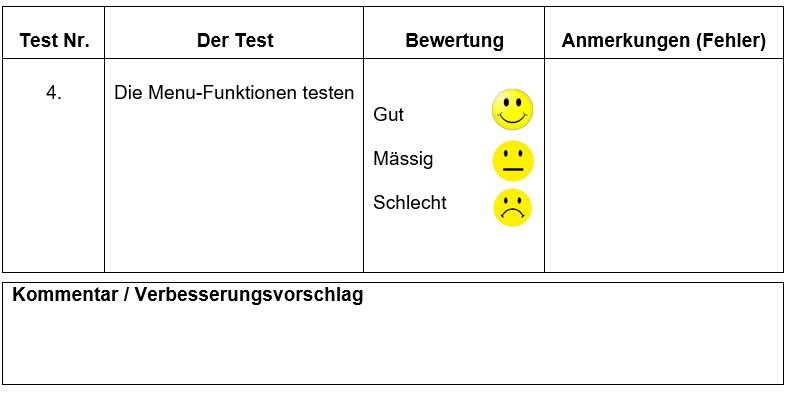
\includegraphics[width=16cm]{Test4.png}
	\label{fig:Test4}
\end{figure}

\begin{figure}[H]
	\centering
	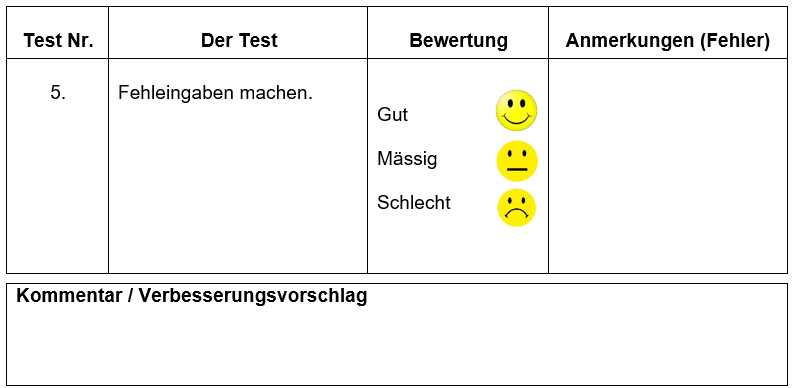
\includegraphics[width=16cm]{Test5.png}
	\label{fig:Test5}
\end{figure}

\begin{figure}[H]
	\centering
	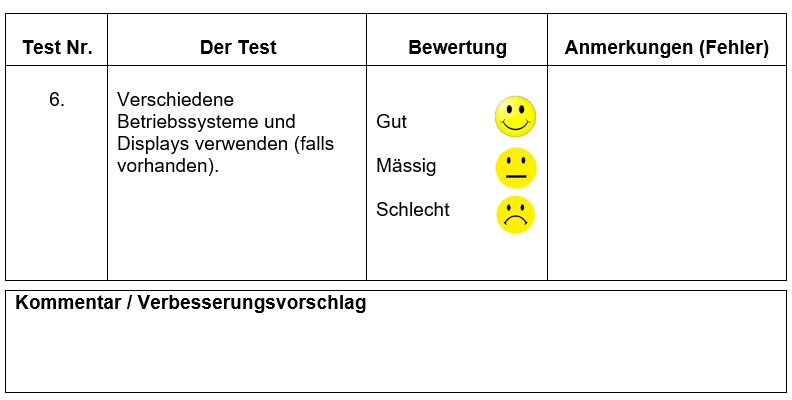
\includegraphics[width=16cm]{Test6.png}
	\label{fig:Test6}
\end{figure}

\begin{figure}[H]
	\centering
	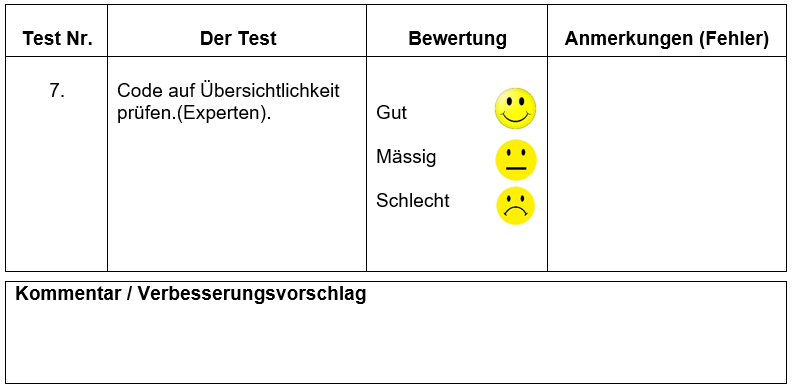
\includegraphics[width=16cm]{Test7.png}
	\label{fig:Test7}
\end{figure}

\begin{figure}[H]
	\centering
	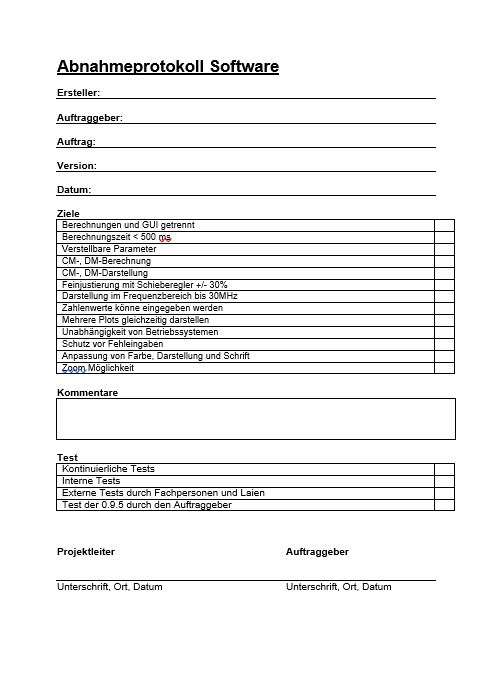
\includegraphics[width=16cm]{Abnahme.png}
	\label{fig:Protokoll}
\end{figure}

%%---NOTES for DEBUG---------------------------------------------------------------------
\ifdraft{%Do this only if mode=draft
%%requires \usepackage{todonotes})
\newpage
\listoftodos[\section{Todo-Notes}]
\clearpage
}
{%Do this only if mode=final
}
\end{document}
